%for a more compact document, add the option openany to avoid
%starting all chapters on odd numbered pages
\documentclass[12pt]{cmuthesis}

% This is a template for a CMU thesis.
% The source for this is pulled from a variety of sources and people.
% Here's a partial list of people who may or may have not contributed:
%
%        bnoble   = Brian Noble
%        caruana  = Rich Caruana
%        colohan  = Chris Colohan
%        jab      = Justin Boyan
%        josullvn = Joseph O'Sullivan
%        jrs      = Jonathan Shewchuk
%        kosak    = Corey Kosak
%        mjz      = Matt Zekauskas (mattz@cs)
%        pdinda   = Peter Dinda
%        pfr      = Patrick Riley
%        dkoes    = David Koes

% some useful packages
\usepackage{times}
\usepackage{fullpage}
\usepackage{graphicx}
\usepackage{amsmath}
\usepackage[numbers,sort]{natbib}
\usepackage[backref,pageanchor=true,plainpages=false, pdfpagelabels, bookmarks,bookmarksnumbered,
%pdfborder=0 0 0,  %removes outlines around hyper links in online display
]{hyperref}
\usepackage{subfigure}
\usepackage{braket}

% Approximately 1" margins, more space on binding side
%\usepackage[letterpaper,twoside,vscale=.8,hscale=.75,nomarginpar]{geometry}
%for general printing (not binding)
\usepackage[letterpaper,twoside,vscale=.8,hscale=.75,nomarginpar,hmarginratio=1:1]{geometry}

\setcounter{secnumdepth}{3}
\setcounter{tocdepth}{3}

% Provides a draft mark at the top of the document.
\draftstamp{\today}{DRAFT}

\usepackage{cleveref}
\crefname{figure}{Figure}{Figures}
\Crefname{figure}{Figure}{Figures}
\crefname{section}{Section}{Sections}
\Crefname{section}{Section}{Sections}
\usepackage{notoccite}

\usepackage{xcolor}
\hypersetup{
    colorlinks,
    linkcolor={red!50!black},
    citecolor={blue!50!black},
    urlcolor={blue!80!black}
}

\usepackage{tikz}
\usepackage{wrapfig}
\usepackage{tabularx}
\usepackage{booktabs}
\usepackage{siunitx}
%\usepackage{setspace}
%\setstretch{1}

\begin {document}
\frontmatter

%initialize page style, so contents come out right (see bot) -mjz
\pagestyle{empty}

\title{ %% {\it \huge Thesis Proposal}\\
{\bf Benchmarking OODA Loop of an Edge-Enabled Autonomous Drone System with On-Board Compute}}
\author{Aditya Chanana}
\date{December 18}
\Year{2024}
\trnumber{}

\committee{
Mahadev Satyanarayanan, Chair \\
Padmanabhan Pillai\\
}

\support{}
\disclaimer{}

% copyright notice generated automatically from Year and author.
% permission added if \permission{} given.

\keywords{edge computing, drones, mobile networks, latency, bandwidth, edge-native applications, computer vision, machine learning}

\maketitle

\begin{dedication}
“Science, my lad, is made up of mistakes, but they are mistakes which it is useful to make, because they lead little by little to the truth.” Jules Verne
\end{dedication}

\pagestyle{plain} % for toc, was empty

%% Obviously, it's probably a good idea to break the various sections of your thesis
%% into different files and input them into this file...

\begin{abstract}

    The "Observe, Orient, Decide, Act" (OODA) loop encapsulates the agility of
    cyber-physical or cyber-human systems that depend on continuous iterations
    of these steps. Systems with faster OODA loops react more quickly to
    changes in their environment. This work extends the SteelEagle
    cloudlet-based autonomous drone system to utilize onboard computational
    abilities. We bechmark the OODA loop of the new setup and identify
    opportunities for optimization. We show how to combine the use of onboard
    computational abilities, for tasks that benefit immensely from a faster OODA loop,
    and offloading, for tasks that are more computationally expensive, leading
    to an optimal system that excels in real-time computer visions tasks.

\end{abstract}

\begin{acknowledgments}
Dave Eckhardt
\end{acknowledgments}



\tableofcontents
\listoffigures

\listoftables

\mainmatter

%% Double space document for easy review:
%\renewcommand{\baselinestretch}{1.66}\normalsize

% The other requirements Catherine has:
%
%  - avoid large margins.  She wants the thesis to use fewer pages,
%    especially if it requires colour printing.
%
%  - The thesis should be formatted for double-sided printing.  This
%    means that all chapters, acknowledgements, table of contents, etc.
%    should start on odd numbered (right facing) pages.
%
%  - You need to use the department standard tech report title page.  I
%    have tried to ensure that the title page here conforms to this
%    standard.
%
%  - Use a nice serif font, such as Times Roman.  Sans serif looks bad.
%
% Other than that, just make it look good...

\chapter{Introduction}
% Goal : 5-10 page talk before the talk
% maybe not 10 pages, but providing a general overview of the paper is the goal here
\section{Motivation}
\label{sec:motivation}
Mobile devices, such as smartphones and smartwatches, have a key limitation---a
limited battery life which allows them to operate for finite periods before
requiring recharging.  Resource-intensive applications, such as those involving
augmented reality or deep learning inference, exacerbate the situation by
accelerating battery depletion.  Consequently, a mobile device cannot match the
sustained performance and resource capacity of stationary computers, which are
free from the requirements of mobility. Mobile devices will always lag behind
static devices in computational ability because of their size and weight
constraints \cite{satya2014}. Increased computational ability, at the same
level of hardware efficiency, demands higher energy consumption. This requires
larger batteries to preserve operating time, thereby increasing weight and
size---which are undesirable for mobile devices.
\Cref{tab:mobility-constraints} shows how mobile devices have lagged behind
servers in computational power over a period of 25 years. This limitation has
been referred to as the ``mobile penalty'', the cost for reduction in
performance required to adhere to mobility constraints
\cite{satya-edge-native}.

\begin{table}[htbp]
    \centering
    \begin{tabular}{@{}lllll}
        \toprule & \multicolumn{2}{c}{\textbf{Typical Server}} & \multicolumn{2}{c}{\textbf{Typical Mobile Device}}\\\midrule
        \textbf{Year} & \textbf{Processor} & \textbf{Speed} & \textbf{Device} & \textbf{Speed}\\\midrule
        1997 & Intel Pentium II & 266 MHz & Palm Pilot & 16 MHz\\
        2002 & Intel Itanium & 1 GHz & Blackberry 5810 & 133 MHz\\
        2007 & Intel Core 2 Quad Q6600 & 2.4 GHz x 4 & Apple iPhone & 412 MHz\\
        2012 & Intel Xeon E5-2690 & 3.8 GHz x 8 & Samsung Galaxy S3 & 1.4 GHz x 4\\
        2017 & Intel Xeon Platinum 8180 & 3.8 GHz x 28 & Google Pixel 2 & 2.35 GHz x 4,\\
             &&&& 1.9 GHz x 4\\
        2022 & AMD EPYC 9654 & 3.7 GHz x 96 & Samsung Galaxy S22 Ultra & 3 GHz x 1,\\
             &&&& 2.5 GHz x 3,\\
             &&&& 1.8 Ghz x 4\\
        \bottomrule
    \end{tabular}
    \begin{captext}
        *While processor efficiency depends on more factors than processor frequency, such as instructions per cycle, it provides a good first-order approximation.
    \end{captext}
    \caption{The Mobility Penalty Over a Period of 25 Years (Adapted from Chen \cite{zchenthesis}, Flinn \cite{flinn2012cyber})}
    \label{tab:mobility-constraints}
\end{table}

Unmanned aerial vehicles (UAVs), or drones, which spend most of their energy on
flight, are particularly affected by this limitation. Larger batteries required
to sustain intensive on-drone computation increases drone weight.  Increased
drone weight leads to an upwards spiral in weight as larger rotors and more
powerful motors are needed to achieve the same amount of lift.  This requires
even larger batteries which, in turn, may require a more reinforced aircraft
structure, and so on. How, then, can we enable mobile devices to do more given
the mobility constraints they are subject to? Advancements in hardware
efficiency provide one possible way forward, but these advancements are slow
and far between. It turns out that there is a way to "cheat" that enables
mobile devices to do more today, leveraging static infrastructure to overcome
the mobility penalty, known as offloading.

A significant body of work in the field of mobile computing has utilized cloud
or cloudlet offloading techniques to address the inherent resource poverty of
mobile devices \cite{satya1996,satya2009}. Cloudlet offload allows mobile
devices to remotely execute computationally expensive tasks on cloudlets that
do not need to be light or small. This allows mobile devices to retain their
low weight and small size, but possess superior computational abilities.

Drones are an excellent category of mobile devices to study because of their
wide range of useful applications as well as their design requirements which
take mobility constraints to the extreme.  We benchmark an autonomous drone
system that leverages offloading techniques to overcome the computational
limitations of consumer-grade drones. We identify its limitations and evaluate
its performance to understand the areas that future work should focus on to
enable more capable drones that can have a wider variety of application.

\section{Overview}
\label{sec:overview}

SteelEagle \cite{bala2024} is an autonomous drone system that leverages
offloading.  Its main tenet is the use of commerical-off-the-shelf (COTS)
drones, which are readily available at low cost but typically have minimal to
no on-board computational resoures.  Utilizing cloudlet offload, SteelEagle
enables COTS drones to perform much more intelligent tasks than what they were
designed for, and exhibit autonomous capabilities typically only found in
larger, more expensive drones.  SteelEagle focuses on active vision tasks which
require the ability to perform live video analytics during flight to determine
the next course of action. SteelEagle drones relay their camera video stream
over a commercial cellular network to a nearby on-ground edge server, a
cloudlet, which runs a computationally expensive pipeline involving neural
networks (\cref{fig:steeleagle-drone-arch}) to perform tasks such as monocular
camera depth perception.  This processing of the raw drone sensor stream allows
obtaining higher level semantic information about the drone's physical
environment. In the case of depth perception, we could infer obstacles that
present the danger of a collision. The drone can then be sent piloting commands
to react, perhaps to actuate to avoid an impending collision.

\begin{figure}[htbp]
\centerline{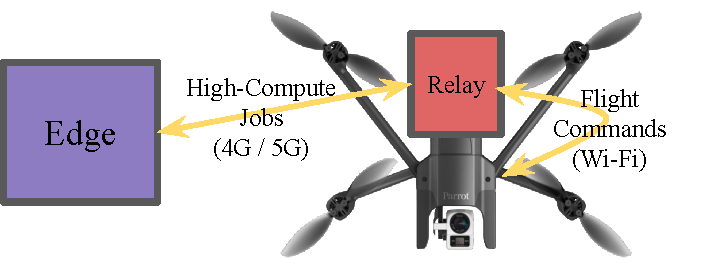
\includegraphics[width = .6\textwidth]{figs/steeleagle-drone-arch-cropped.pdf}}
\caption{Cloudlet Offload in SteelEagle}
\label{fig:steeleagle-drone-arch}
\end{figure}

An important consideration for SteelEagle is the agility of the resulting
system.  How quickly can a drone respond to a change in its environment? The
end-to-end latency of the entire execution pipeline, including sensing,
offloading, inferencing, decision making, and actuation, defines the agility. A
high end-to-end latency can severely handicap the drone---it must fly at a
higher altitude or at lower speeds to be safe if it takes a long time to
identify obstacles and actuate to avoid them. Drone flight at a higher altitude
precludes close observation, and lower speeds make missions take longer,
limiting the capabilities of the drone. Search and rescue missions in forests,
and missions to aid law enforcement operations in dense cities, for instance,
must fly at low altitudes while avoiding obstacles in the environment that
present a collision risk---trees branches, streetlight poles, utility wires,
and buildings---without impacting mission speed. Unless we can achieve high
agility, SteelEagle drones will struggle to perform these missions well.  Since
these missions are one of the most compelling use cases for autonomous drones,
benchmarking the end-to-end pipeline to determine latency bottlenecks and
identifying opportunities for latency optimization is a very worthy pursuit.

SteelEagle drones currently perform no onboard computation---they are
controlled exclusively over the network.  While this strategy allows treating
consumer-grade non-programmable drones as black boxes, it presents severe
limitations. First, SteelEagle drones struggle in areas with unreliable cell
service and are completely inoperable in regions without cellular coverage.
Second, cloudlet offload imposes an upper bound on drone agility as it adds the
cost of a round-trip latency to a cloudlet. As originally envisioned, cloudlets
are differentiated from clouds because of their network proximity, which allows
application end-to-end response time to be just a few milliseconds. In
practice, the usage of commerical cellular networks for offload to the cloudlet
increases this latency to tens of milliseconds. This limits the agility of the
drone, as the reaction time is at least the round-trip time to the cloudlet.

This thesis performs a comprehensive benchmarking of the SteelEagle system,
revealing the current system bottlenecks and identifying opportunities for
optimization. In recent years, domain-specific system-on-a-chip devices have
become available that provide substantial energy-efficient on-board
computational resources through the inclusion of hardware accelerators in the
chip design. These chips can decode the video stream generated by the drone and
perform analytics using TensorFlow Lite models, and often include 5G and Wi-Fi
connectivity. Using such a chip as a payload on SteelEagle drones allows us to
continue treating the drone as a black box, but employ new cloudlet offload
tactics that result in tighter OODA loops for use cases that can utilize the
hardware accelerators, while retaining the generality offered by cloudlet
offload. We explore the use of onboard computation to mitigate the limitations
of SteelEagle, and explore the resulting impact on drone agility.

\section{Contributions}

The contributions of this thesis include
\begin{itemize}
  \item A discussion of efforts to optimize SteelEagle that yielded a two-fold
      improvement in drone-to-cloudlet latency
  \item A mapping of the SteelEagle pipeline to the OODA loop framework
  \item An analysis of the SteelEagle pipeline's performance from a latency
      and bandwidth perspective
  \item An evaluation of the use of an onboard computation device to improve
      SteelEagle performance and alleviate its limitations
\end{itemize}

\section{Organization}
\Cref{ch:background} provides a detailed background on edge computing and the
SteelEagle autonomous drone system. \Cref{ch:uav-primer} describes the history
of drones and their development over time. We discuss the applications that
drones are used in today, as well as the capabilities of today's drones.  We
also discuss what autonomy means for drones. In
\cref{ch:optimizing-steeleagle}, we describe our experimental setup for
measuring the latency of the SteelEagle system. We include measurements which
provided the insight needed to optimize SteelEagle, allowing for a two-fold
improvement in SteelEagle's drone-to-cloudlet latency. In \cref{ch:voxl}, we
explore the use of an onboard computation device called the Modal AI VOXL to
augment SteelEagle. We conclude with \cref{ch:conclusion}, presenting
concluding remarks and providing a road map for future work.


\begin{comment}
The "Observe, Orient, Decide, Act" (OODA) loop framework devised by military
strategist John R. Boyd provides a framework to structure our investigation
into the end-to-end latency of SteelEagle. According to Boyd, decision-making
happens in a continuous iteration of these steps. Boyd attributed the faster
OODA loop of U.S. pilots flyng F-86s, because of the bubble-shaped canopy
offering better visibility and hydraulic controls that allowed for easier
switching between manoeuvres, as the reason the slower F-86s fared better than
the North Korean MiG-15s during the Korean War \cite{morton1995}. A system with
a tighter OODA loop corresponds to a more agile drone. Instead of measuring
just the overall system latency, performing a break down of the latency across
the OODA steps provides more insight into system latency bottlenecks.
\end{comment}

\chapter{Primer on UAVs}

\section{History of Drones}
\label{sec:drone-history}

Unmanned aerial vehicles (UAVs), or drones, are aircraft that can be operated
remotely without the need for a human pilot on board. While there were many
early pilotless aircraft, the first remote controlled aircraft appeared during
the First World War, developed by Britain and the US in 1917
\cite{dronehistory}. Many of these early drones were used as anti-aircraft
gunnery training targets. In the 1930s, the term "drone" arose inspired by the
de Havilland DH82B Queen Bee (\cref{fig:queen-bee}), designed as a low-cost
radio-controlled target aircraft, which saw over four hundred units built by
1943. The Queen Bee was the first drone designed with the ability to return to
ground safely and be reused \cite{queenbee, pbs05}.

\begin{figure}[htbp]
\centerline{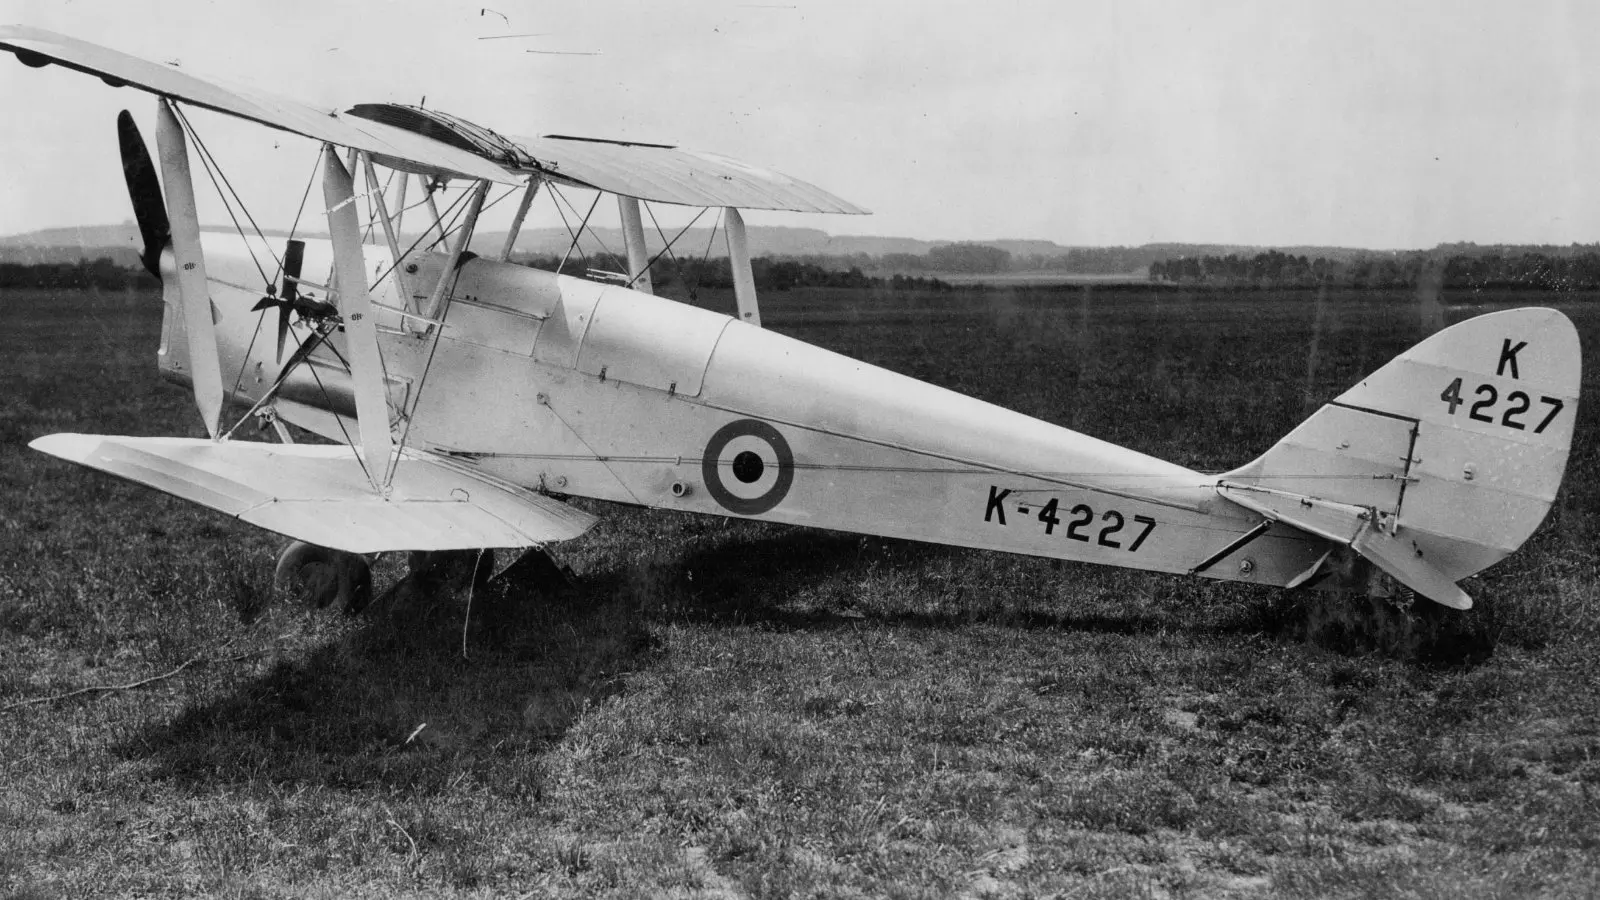
\includegraphics[width = .6\textwidth]{figs/queenbee.png}}
\caption{de Havilland DH82B Queen Bee \cite{baesystems}, the first radio-controlled drone}
\label{fig:queen-bee}
\end{figure}

These early drones were fixed-wing aircraft that were used primarily for combat
or training. From the 1970s, drones such as the Ryan Model 147 Lightning
Bugdrones were developed for use in surveillance missions. These drones carried
a camera and could fly for hours at high altitude \cite{pbs12}. The Pioneer
UAV, introduced in 1986, saw extensive use in the Gulf War. Today, the General
Atomics MQ-1 Predator can fly for over 14 hours performing surveillance
missions using an array of sensors, including infrared cameras.

\begin{figure}[htbp]
\centerline{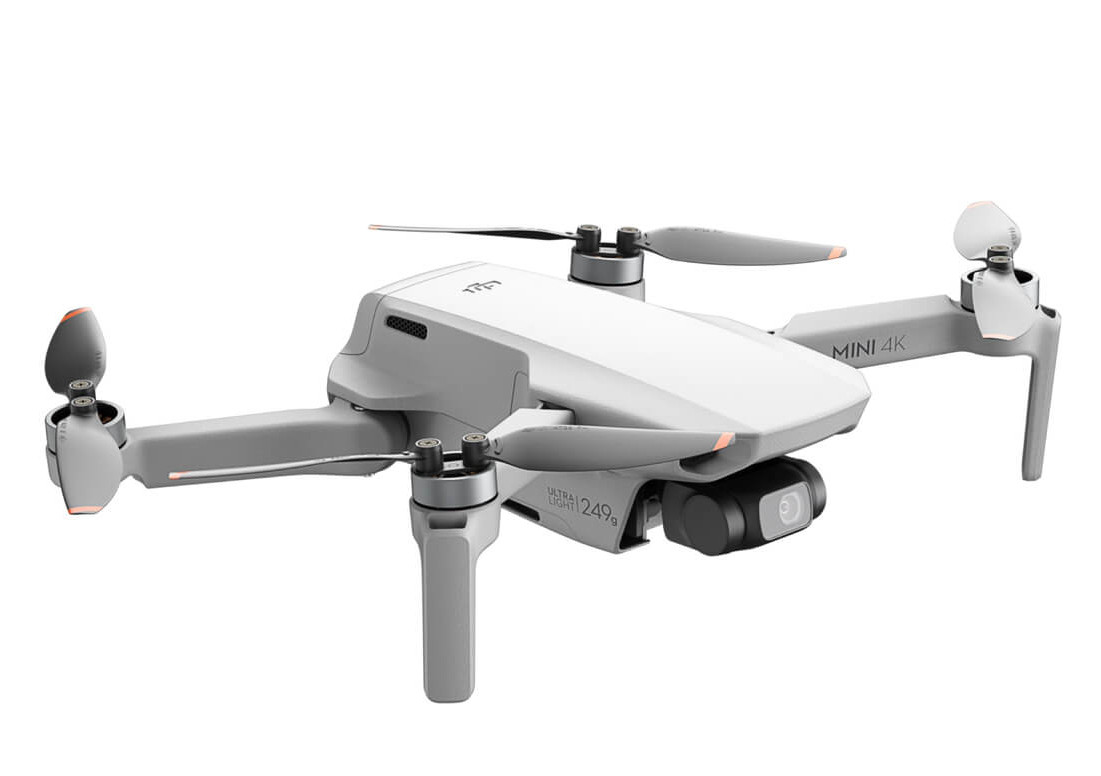
\includegraphics[width = .4\textwidth]{figs/dji-mini-4k.jpg}}
\caption{DJI Mini 4K}
\label{fig:dji-mini-4k}
\end{figure}

The turn of the century saw the use of small drones in civillian settings, with
technology advances making them cheaper to produce. Drones, particularly
quadcopters (\cref{fig:dji-mini-4k}), started being used for mapping, aerial
photography, industrial inspections and security, and precision agriculture
\cite{giones2017}. Compared to previous fixed-wing military drones, quadcopters
offer superior maneuverability and the ability to hover. They utilize four
motor-rotors, with two spinning clockwise and the other two counterclockwise.
Variations in motor speed allow for precise hovering and maneuverability. This
makes quadcopter drones well-suited for both indoor and outdoor use.  Since the
2010s, drones have evolved significantly, with a range of consumer photography
and racing drones easily available to consumers, at a wide range of price
points. Drones are commonly used for filming and recreation, and have also seen
use in logistics, to deliver packages. They have also been put to use in search and rescue
\cite{scherer2015}\cite{tomic2012}\cite{mcrae2019} and wildlife conservation \cite{gemert2015}\cite{gonzalez2016}.

The scale of their adoption is
immense---The Federal Aviation Administration (FAA) has received registrations
for almost 800,000 drones \cite{faa_drones_2024}.  This figure excludes
thousands of hobbyist drones weighing under 250 g that do not require FAA
registration.

\section{Capabilities of Today's Drones}
\label{sec:drone-capabilities}

Today, the set of features available in consumer-grade drones is impressive.
The DJI Mini 4K (\cref{fig:dji-mini-4k}) is priced at \$299, weighs under 250g,
records video at 4K 30 FPS, and has a maximum flight time of about 30 minutes
\cite{dji_mini_4k}. Most drone's today have the ability to fly
semi-autonomously in addition to the ability to be controlled remotely by a
human. As shown in \cref{fig:drone-components}, drones have advanced
microprocessors that abstract away the lower-level mechanics of quadcopter
drone flight. Components such as the Electronic Speed Controller (ESC) enable
precise control of the drone's brushless electric motors. On-board positioning
systems such as Global Navigation Satellite System (GNSS) receivers give the
drone the ability to navigate between waypoints.  Using inputs from on-board
intertial measurement unit (IMU) sensors such as gyroscopes, accelerometers,
and magnetometers, drones can determine their orientation, acceleration, and
rotation, allowing them to adjust their motors in real-time to counter wind and
hover in a fixed position. They can also typically takeoff and land
autonomously. On-board flight control software such as PX4 or ArduPilot, also
known as an "autopilot," makes these higher-level functions possible, taking
inputs from the IMU and GNSS sensors and outputting control commands to the
ESC.

\begin{figure}[htbp]
\centerline{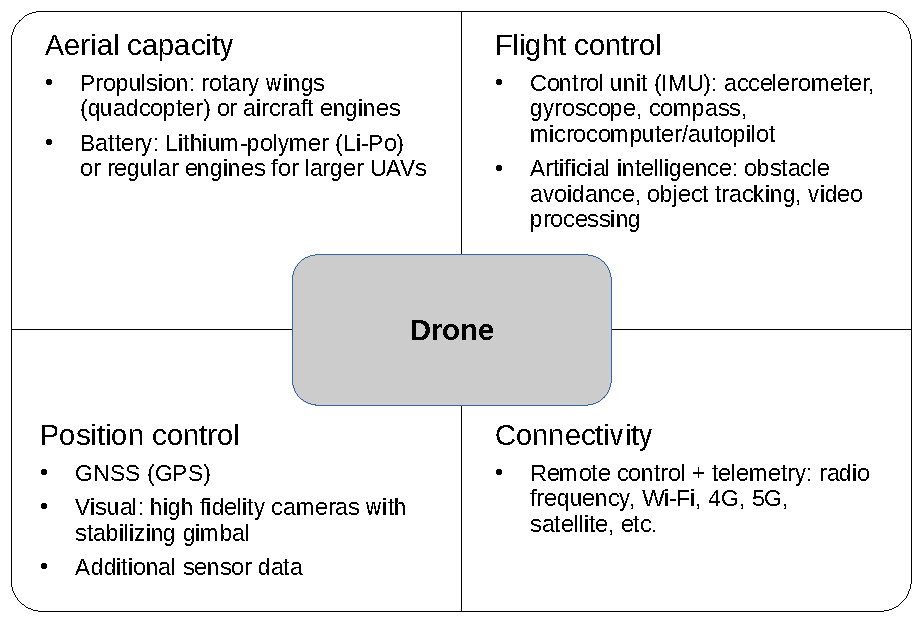
\includegraphics[width = .6\textwidth]{figs/drone-components-crop.pdf}}
\caption{Components of a drone \cite{giones2017}}
\label{fig:drone-components}
\end{figure}

Drones are equipped with a variety of cameras, such as monocular and stereo.
Monocular cameras capture images and videos from a single point of view, and
are common in consumer aerial photography drones. Monocular cameras are often
mounted on a gimbal, which stabilizes the drone's camera during motion and also
allows the ability to capture different viewing angles through gimbal motion.
Stereoscopic cameras, on the other hand, offer multiple point of views. Having
more than one camera allows the use of epipolar geometry and triangulation to
determine distance from objects efficiently, and perform obstacle avoidance.
The DJI Mini 4 Pro, for instance, has multiple binocular cameras, facing
forward, backward, sideways, upwards, and downwards. This allows the Mini 4 Pro
to perform omnidirectional obstacle sensing. During manual pilot flight, the
drone offers pilot assistance features that stop the drone if it is headed for
an imminent collision, and also provide the option to circumvent obstacles
automatically altogether. Drones equipped with monocular cameras typically lack
these advanced obstacle avoidance systems, but are cheaper and more common.

While consumer-grade drones offer many semi-autonomous features, complex
fully-autonomous features are limited to more expensive commerical drones.  For
example, a consumer drone could be instructed to navigate to a given GPS
coordinate or, in some advanced drones, even track an on-ground target. But
complex missions, such as patrolling a set of waypoints while searching for an
on-ground target, and transitioning to track the target once it is detected,
remain out of the reach of consumer drones.

Consumer drones are typically controlled over Wi-Fi using a controller or a
smartphone app, and typically lack cellular connectivity, limiting their
flying range.

\section{Levels of Autonomy}

\begin{figure}[htbp]
\centerline{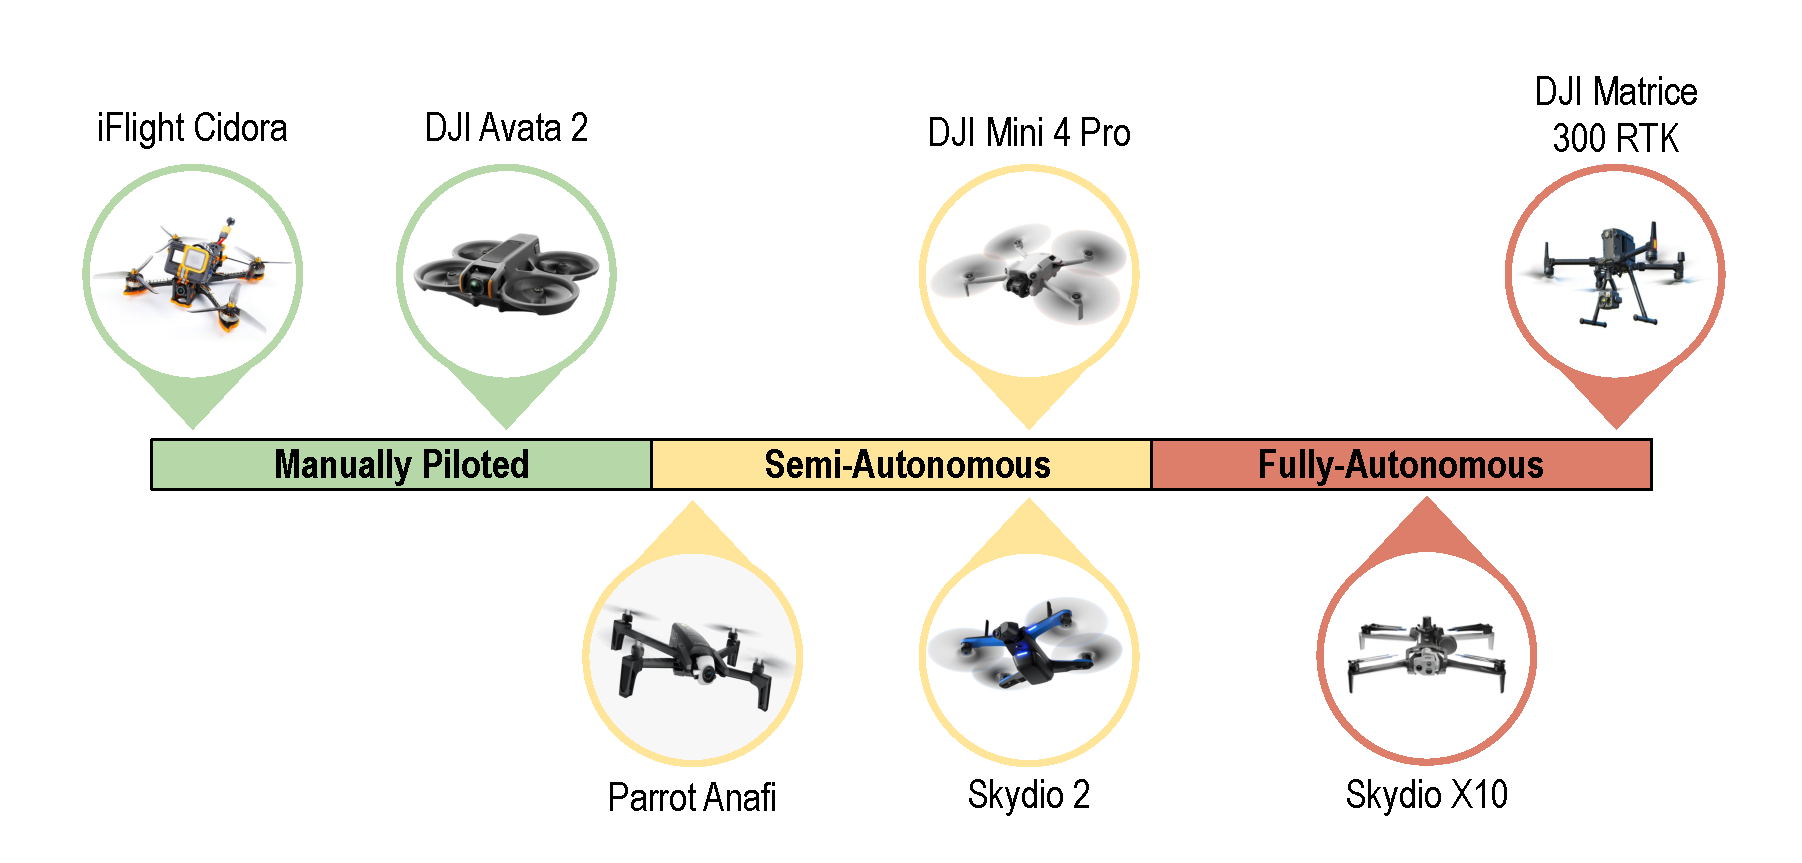
\includegraphics[width = .8\textwidth]{figs/autonomy-spectrum.pdf}}
\caption{Drone Autonomy Levels}
\label{fig:drone-autonomy-spectrum}
\end{figure}

Drones exhibit varying levels of autonomy, as shown in
\cref{fig:drone-autonomy-spectrum}. As we move to the right, the reliance on
human drone operators reduces, as the drones feature more autonomous abilities.
On the manual end of the spectrum are drones such as the DJI Avata 2, a
first-person view (FPV) drone. FPV drone pilots receive a real-time video
stream from the drone's onboard camera and manually control the drone. These
drones are optimized for high-speed flight and maneuverability, giving them the
ability to navigate through tight obstacles at speed. Manually piloting a drone
requires skill and constant human pilot input, which reduces the usefulness of
these drones.

Drones such as the Parrot Anafi include semi-autonomous features such as the
ability to hover and navigate between waypoints. These drones often include a
return-to-home (RTH) function which automatically returns the drone to its
takeoff location if the battery is low, or if the drone loses its connection to
the pilot's controller. Advanced semi-autonomous drones such as the DJI Mini 4
Pro can also follow a human or vehicle target. These semi-autonomous features
reduce the level of skill required for piloting and the reliance on the human
pilot, but still require the pilot to specify the next course of action to
fulfill higher-level mission objectives.

\begin{figure}[htbp]
    \centerline{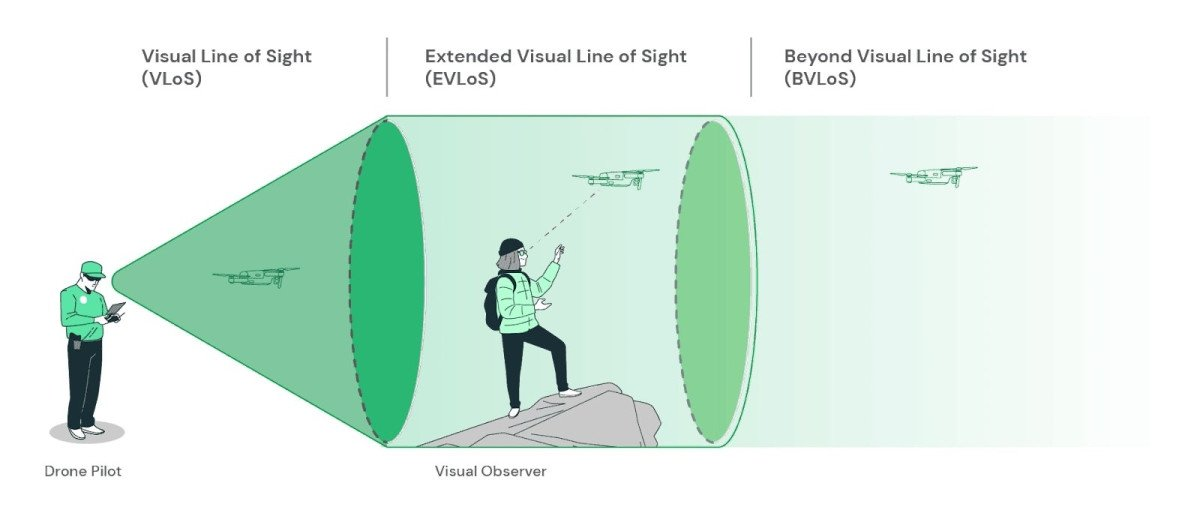
\includegraphics[width = .9\textwidth]{figs/BVLOS.jpeg}}
    \caption{Drone Operation Line-of-Sight Requirements \cite{flyeye_bvlos}}
\label{fig:drone-line-of-sight}
\end{figure}

On the right end of the spectrum are fully-autonomous drones, which execute a
pre-programmed mission without a human pilot while adapting to operational and
environmental conditions during flight. The DJI Matrice 300 RTK, for instance,
can inspect pre-specified objects of interest, such as power transmission
towers, without any human input.

Regulatory hurdles, however, impact the versatility of fully-autonomous drones.
FAA regulations require that drone operators keep drones within sight during
flight \cite{faa_part107}. For FPV drones, it is sufficient to have a visual
observer that always has the drone in sight.  These two modes of operation
correspond to ``Visual Line of Sight'' (VLoS) and ``Extended Visual Line of
Sight'' (EVLoS) in \cref{fig:drone-line-of-sight}. While a number of use cases
can be covered under these modes of operation, the holy grail for drones lies
in ``Beyond Visual Line of Sight'' (BVLoS) operation. BVLoS operation allows
drones to fly a much wider range of missions. Missions involve package delivery
requires drones to fly to a far-off destination, improving speed and reducing
the logistical cost compared to human delivery via road. Requiring a human
observer to maintain sight of the drone at all times defeats the purpose of
this application.

\chapter{Optimizing SteelEagle Performance}
\label{ch:optimizing-steeleagle}

As explained in \cref{sec:overview}, the performance of the SteelEagle system
determines its versatility. A drone that is slow to react will be unable to
effectively navigate obstacle-dense environments. The chances of the drone
losing track of a fast on-ground target that is moving erratically increases
substantially if the drone is slow in keeping the target centered in its view.
Given the importance of performance, this chapter details how performance is
defined for SteelEagle, how it is measured, and work done to identify
performance bottlenecks and optimize the system.

\cref{sec:exp1} describes initial efforts to optimize the system that yielded a
more than two-fold reduction in drone-to-cloudlet latency, discovering negative
scale-out attributes of FFmpeg, a video decoding library.  \cref{sec:exp2}
describes subsequent efforts to establish a more systematic approach to
profiling SteelEagle, which found the encoding of the RTSP video stream
generated by the drone to be the biggest contributor to latency.

\begin{figure}[htbp]
\centerline{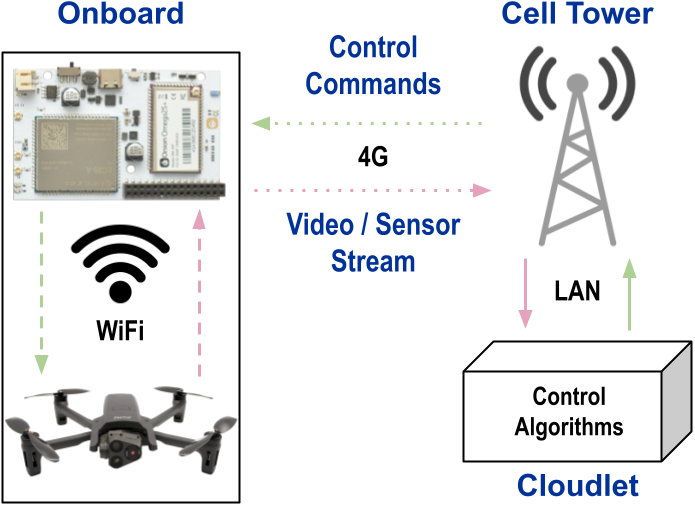
\includegraphics[width = .5\textwidth]{figs/fig-simplified-arch.png}}
\caption{SteelEagle Edge Offload Pipeline}
\label{fig:simplified-arch}
\end{figure}

\section{How is Performance Defined in SteelEagle?}
\label{sec:steeleagle-performance-def}

The performance of SteelEagle is determined by the end-to-end latency and
throughput of the system. Currently, SteelEagle drones function as thin
clients, with the use of a communications relay to make up for the lack of
cellular connectivity on commerical-off-the-shelf (COTS) drones. The sensor
stream from the drone is forwarded to the communications relay over Wi-Fi,
which in turn forwards it to the cloudlet over 4G LTE. After performing
inference on the received data, the cloudlet sends back piloting commands to
the drone, via a hop through the communications relay
(\cref{fig:simplified-arch}). As a result, the end-to-end performance is
determined by several components of the pipeline:
\begin{enumerate}
    \item[(a)] \textbf{On-drone sensing.} Capture of images by the drone's camera
    \item[(b)] \textbf{On-drone pre-processing.} Pre-processing of sensor data.
        For example, generation of video stream from raw camera images
    \item[(c)] \textbf{Transmission to cloudlet.} Offloading to cloudlet to
        perform resource-intensive computation
    \item[(d)] \textbf{Cloudlet processing.} Inferencing, planning, and decision
        making based on sensor data
    \item[(e)] \textbf{Transmission to drone.} Transmission of actuation command
        back to the drone
    \item[(f)] \textbf{Drone post-processing.} Drone processing to interpret
        command
    \item[(g)] \textbf{Drone actuation.} Electromechanical actuation of drone's
        motors
\end{enumerate}

Each of these components has a latency associated with it, and a throughput
that it is capable of. The performance of components (a), (b), (f), and (g) is
fixed for a given drone. Factors such as the drone camera's sensor readout time
and shutter speed used affect the frame capture latency, and thus determine the
performance of component (a). Component (b) consists of any processing of the
sensor data before it is transmitted from the drone. The generation of an H.264
stream, for instance, adds latency since the compression process is
computationally intensive, involving analysis of deltas between successive
frames.

For components (c) and (e), performance is determined by the cellular network
used for communication between the relay and the cloudlet. While there is
variance associated with the performance of these components, factors such as
the number of network hops, distance between the relay to the cloudlet, and the
network signal strength available to the relay largely determine the 99th
percentile value of their latency and throughput over a longer period of time.
The performance of component (d) can vary largely based on whether decoding of
the drone stream data is required and type of inferencing that is performed. A
DNN with a complex architecture, for instance, can take much longer for
inference than a traditional computer vision approach. The same inference can
also take less time on a more powerful cloudlet.

\begin{figure}[htbp]
\definecolor{observe-color}{RGB}{175,208,149}
\definecolor{orient-color}{RGB}{255, 255, 166}
\definecolor{decide-color}{RGB}{255,170,149}
\definecolor{act-color}{RGB}{224,194,205}
\centering
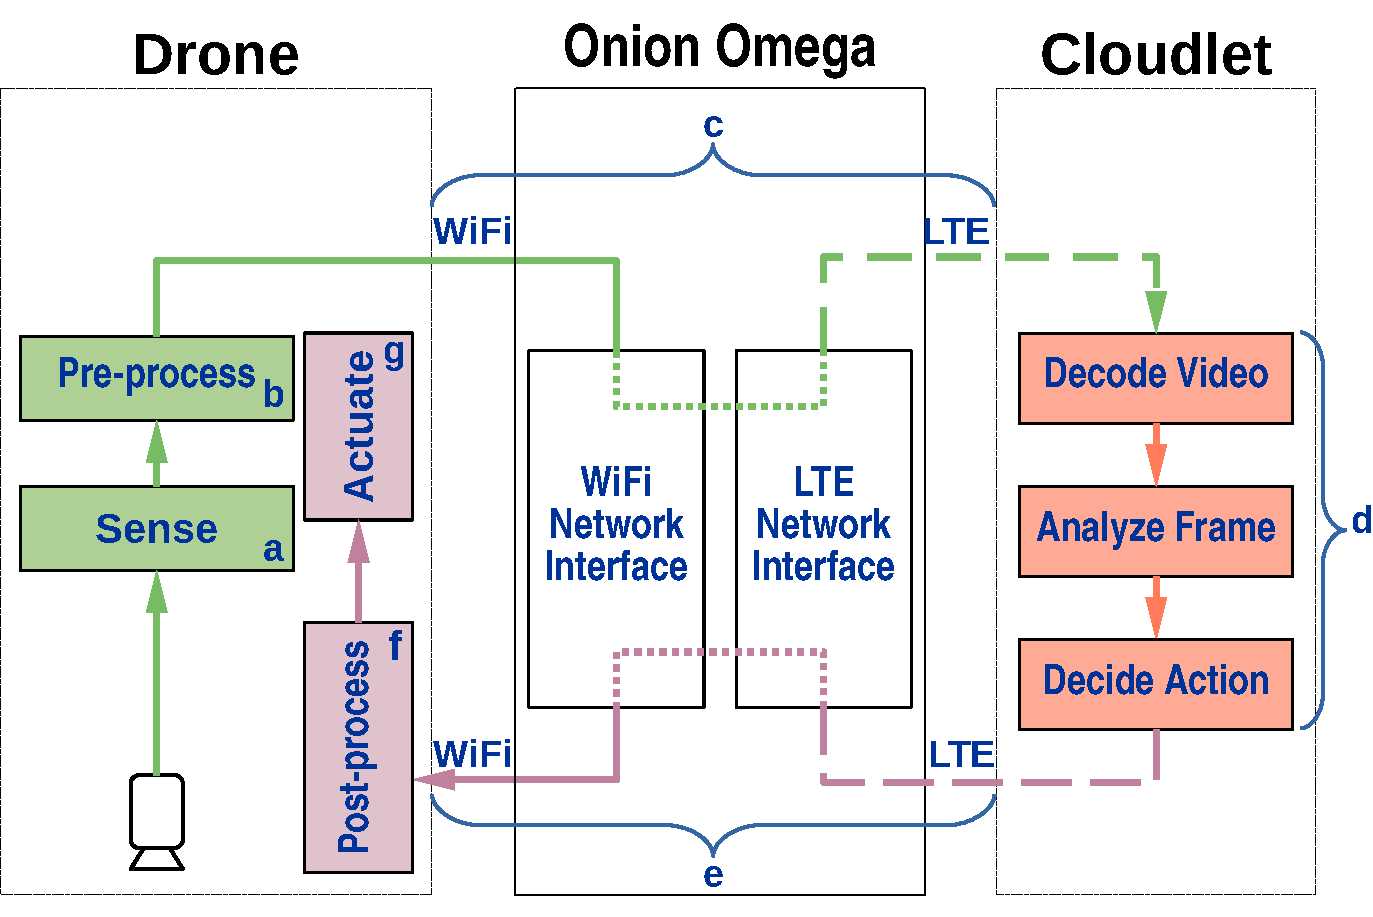
\includegraphics[width = .6\textwidth]{figs/fig-ooda-loop.pdf}\\
\begin{tikzpicture}
    \draw[fill=observe-color] (1.0,0) rectangle (1.3,0.3);
    \node[right] at (1.3,0.15) {\small Observe};

    \draw[fill=decide-color] (2.9,0) rectangle (3.2,0.3);
    \node[right] at (3.2,0.15) {\small Orient \& Decide};

    \draw[fill=act-color] (6.1,0) rectangle (6.4,0.3);
    \node[right] at (6.4,0.15) {\small Act};
\end{tikzpicture}
\caption{Mapping the SteelEagle pipeline to the OODA loop}
\label{fig:ooda-mapping}
\end{figure}

\Cref{fig:ooda-mapping} shows how these components can be mapped to the various
stages of the OODA loop framework, defined in \cref{sec:ooda-loop}. The
``Observe'' phase includes components (a), (b), and (c). Components (d) maps to
the ``Orient'' and ``Decide'' phases. Finally, components (e), (f), and (g)
correspond to the ``Act'' phase.

\section{Measuring the Performance of the SteelEagle Pipeline}
\label{sec:steeleagle-performance-measurement}

Benchmarking the performance of SteelEagle is challenging since it uses COTS
drones that restrict modification of its onboard software. The inability to add
software instrumentation on the drone makes it difficult to determine when a
given frame was transmitted from the drone. To circumvent this restriction,
Bala et al adapted the technique George et al used for measuring
motion-to-photon latency in augmented reality \cite{george20}.


\begin{figure}[htbp]
\centerline{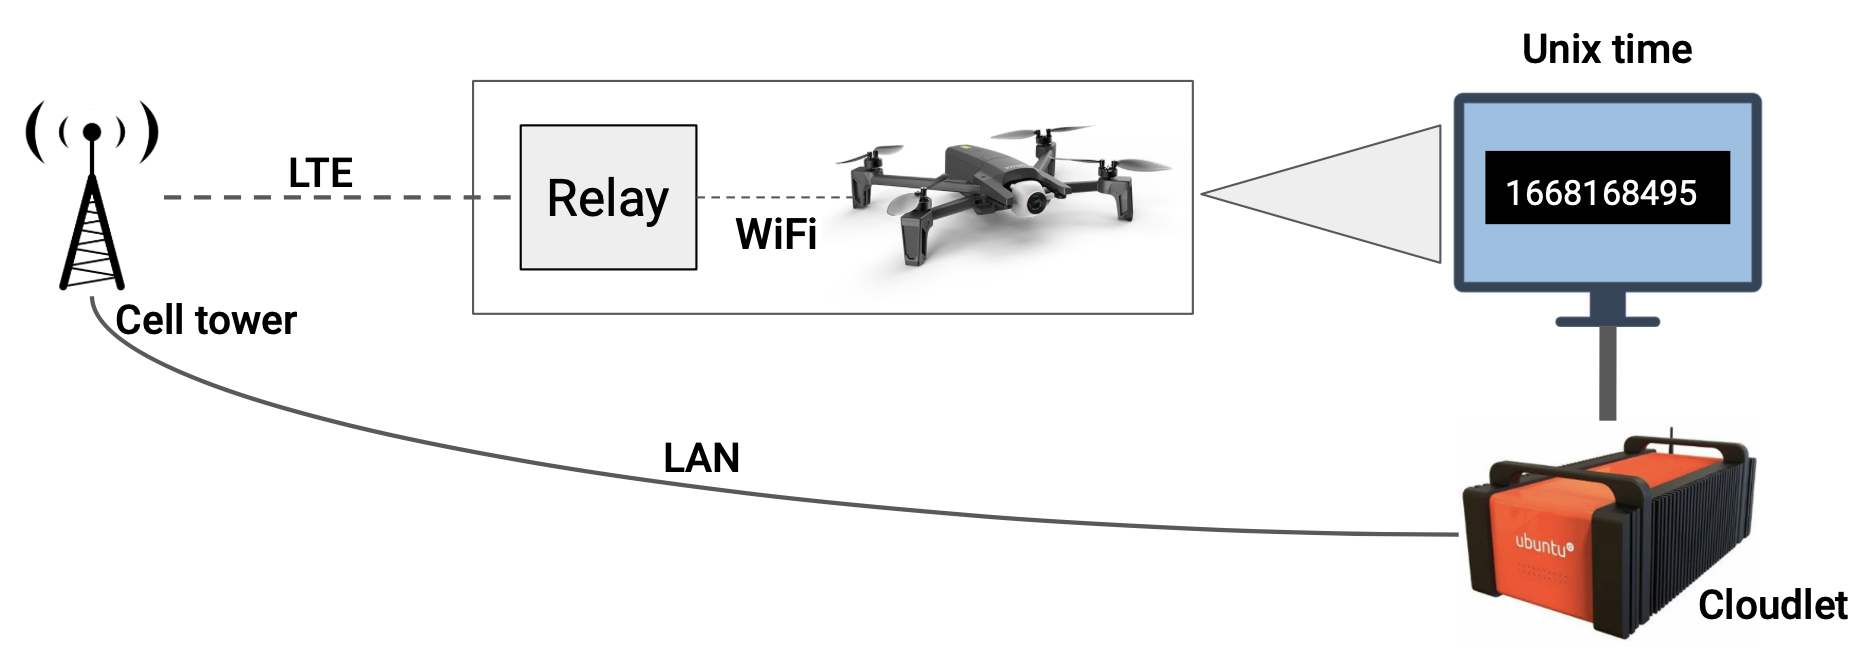
\includegraphics[width = .8\textwidth]{figs/mtp_pipeline.png}}
\caption{Technique for measuring end-to-end latency}
\label{fig:latency-measuring-technique}
\end{figure}
As shown in \cref{fig:latency-measuring-technique}, the drone is kept
stationary in a lab setting with its camera pointed at a display connected to
the cloudlet showing the current Unix timestamp at millisecond granularity. The
drone captures images containing the timestamp displayed and transmits them to
the cloudlet through the SteelEagle pipeline. The cloudlet records the
timestamp at which it receives each frame, storing the frame along with this
timestamp. These saved frames are then
post-processed to compute the difference between the timestamps shown in each
frame and the timestamps at which they were received at the cloudlet. This
difference corresponds to the latency of components (a) through (d).

\section{Optimizing SteelEagle Video Decoding}
\label{sec:exp1}

\begin{figure}[htbp]
\centerline{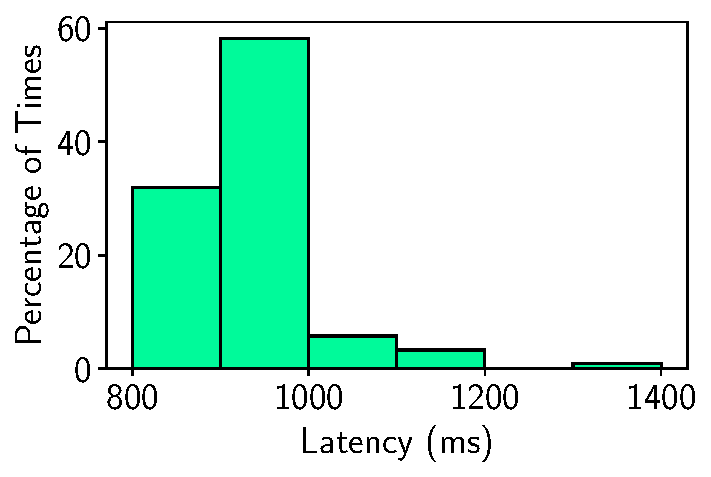
\includegraphics[width = .4\textwidth]{figs/bala_latency.pdf}}
\caption{Original SteelEagle Latency \cite{bala2024}}
\label{fig:steeleagle-original-latency}
\end{figure}

\begin{figure}[b]
    \centering
    \begin{subfigure}[t]{0.45\textwidth}
        \centering
        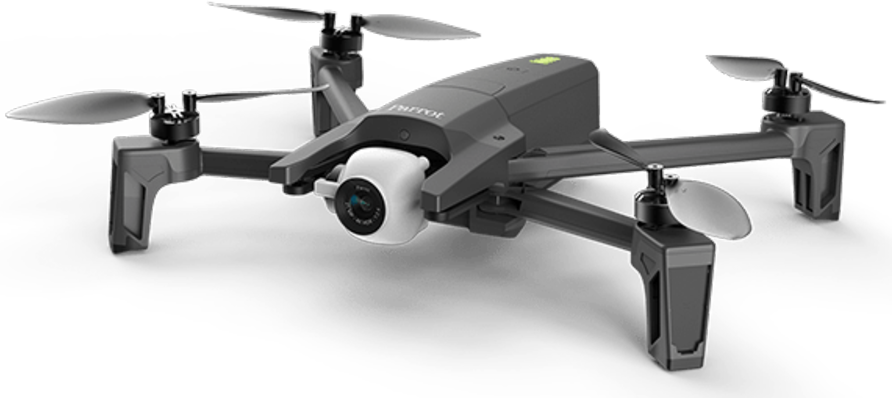
\includegraphics[height=1in]{figs/parrot-anafi.pdf}
        \caption{Parrot Anafi}
        \label{fig:parrot-anafi}
    \end{subfigure}
    \begin{subfigure}[t]{0.45\textwidth}
        \centering
        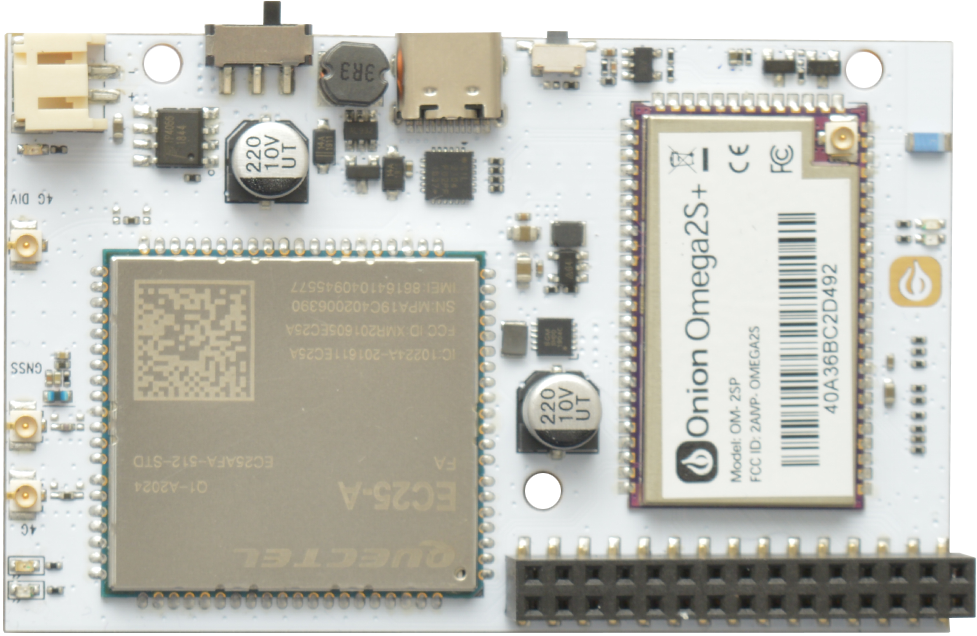
\includegraphics[height=1in]{figs/onion-omega.png}
        \caption{Onion Omega}
        \label{fig:onion-omega}
    \end{subfigure}
    \caption{The commerical-off-the-shelf components used in the SteelEagle system}
\end{figure}

The starting point of our investigation into the performance of the SteelEagle
system is the mean drone-to-cloudlet latency of 933 ms reported by Bala et al
in their benchmarking of the SteelEagle system
(\cref{fig:steeleagle-original-latency}). This includes the ``Observe'' and
``Orient \& Decide'' components of the OODA pipeline, components (a) through
(d) in \cref{fig:ooda-mapping}.  The latency was obtained using the Parrot
Anafi drone (\cref{fig:parrot-anafi}), which transmits a 720p H.264 RTSP stream
at 30 FPS over UDP from its monocular camera.  The Anafi uses a slice encoding
and intra-refresh scheme that disperses keyframe slices across multiple network
packets \cite{anafi_white_paper}. To reduce network bandwidth requirements, it
generates an H.264 compressed video stream using onboard hardware from the raw
frames that it obtains from its camera. Consequently, decoding of this H.264
stream is required to obtain individual video frames.  The setup uses the Onion
Omega 2 LTE (\cref{fig:onion-omega}) as a network gateway to allow the Anafi to
reach the cloudlet over LTE, since the Parrot Anafi lacks cellular
connectivity.

The technique to measure latency described in
\cref{sec:steeleagle-performance-measurement} does not provide a granular
latency breakup. As a result, it is not clear from the measurements where the
bottleneck resides. As an initial approach, we measure the impact on latency
when the cloudlet location and the video decoding library used are modified. If
the latency is significantly reduced by changing a factor, we can conclude that
the bottleneck resides in the corresponding component.

\subsection{Experimentation Parameters}

Our first experiment measures the impact on latency when the location of the
backend and the video decoding library used is changed.
\Cref{tab:experiment-parameters} summarizes the different parameters tested
along these dimensions.
\begin{table}[htbp]
    \centering
    \caption{Latency Pipeline Experimentation Parameters}
    \label{tab:experiment-parameters}
    \begin{tabular}{@{}ll@{}}
        \toprule
        \textbf{Dimension} & \textbf{Parameters} \\ \midrule
        Backend Location & Cloudlet, AWS Small, AWS Big \\
        Video Decoding Library & FFmpeg, PDrAW \\ \bottomrule
    \end{tabular}
\end{table}

We now describe the details of these parameters:

\begin{itemize}

    \item \textbf{Location of backend.} Three backend locations with different
specifications, each offering varying levels of performance, are considered to
evaluate how hardware scale-up affects system latency. The SteelEagle backend
is either set up on a bare-metal server on CMU's campus, labeled ``Cloudlet'',
or on an EC2 VM in AWS East (Virginia). Two types of EC2 instances are used,
``AWS Small'' and ``AWS Big''. The CMU Cloudlet has two
Intel\textsuperscript{\textregistered} Xeon\textsuperscript{\textregistered}
E5-2699 v3 CPUs clocked at 2.30 GHz for a total of 72 vCPUs, 128GB main memory,
and an NVIDIA\textsuperscript{\textregistered}
GeForce\textsuperscript{\textregistered} GTX 1080 Ti GPU. AWS denotes a
\texttt{g4dn.xlarge} EC2 instance which has 4 vCPUs, 16GB of memory, and an
NVIDIA T4 GPU. AWS Big is a \texttt{g4dn.16xlarge} EC2 instance which has 64
vCPUs, 256GB main memory, and also an NVIDIA T4 GPU. \Cref{tab:backend-specs}
summarizes these specifications.

\begin{table}[h]
    \centering
    \caption{Specifications of Backends Used in Experiment}
    \label{tab:backend-specs}
    \begin{tabular}{@{}llll@{}}
        \toprule
        \textbf{Backend} & \textbf{vCPUs} & \textbf{Memory} & \textbf{GPU} \\ \midrule
        AWS Small & 4 & 16 GB & NVIDIA\textsuperscript{\textregistered} T4\\
        AWS Big & 64 & 256 GB & NVIDIA\textsuperscript{\textregistered} T4\\
        Cloudlet & 72 & 128 GB & NVIDIA\textsuperscript{\textregistered} GeForce\textsuperscript{\textregistered} GTX 1080 Ti\\
        \bottomrule
    \end{tabular}
\end{table}

\item \textbf{Video decoding library.} Two video decoding libraries are considered:
FFmpeg and PDrAW (pronounced ``pedro''). FFmpeg \cite{ffmpeg} is an open-source
project that offers libraries for video encoding/decoding and
multiplexing/demultiplexing. FFmpeg is known for forming a core part of the VLC
media player. We interact with FFmpeg through OpenCV~\cite{opencv}, which
offers the ability to use FFmpeg as a backend for its video capture APIs.
PDrAW \cite{pdraw} is a part of Parrot's Ground SDK software. Similar to
FFmpeg, it includes multiplexing/demultiplexing abilities and can read from the
RTSP stream generated by the Parrot Anafi drone. Unlike FFmpeg, however, PDrAW
is intended as a video player for RTSP and MP4 videos and lacks general-purpose
encoding and decoding abilities.

\end{itemize}
\subsection{Experimental Results}

\Cref{tab:latency_summary} summarizes the results obtained. For each backend
location, the latency is measured using the two different video decoding
libraries. The mean latency of 933 ms obtained by Bala et al mentioned before
used FFmpeg with the ``Cloudlet'' backend. We measured a lower mean of 888 ms
using these parameters because our experiments do not include inference time on
the cloudlet. Inference time can vary across different machine learning models,
depending on the kind of pre-preprocessing performed and architectural details
such as the number of hidden layers used in deep neural networks.  Not
including inference time, then, allows us to focus on the contribution of other
components.

\begin{table}[ht]
    \centering
    \caption{Drone-to-Cloudlet SteelEagle Latency (in ms)}
    \label{tab:latency_summary}
        \sisetup{
        detect-all,
        table-number-alignment = center,
        input-decimal-markers = {.},
        group-separator={,},
        group-minimum-digits=4
    }
    \begin{tabularx}{0.6\linewidth}{@{}
        X
        c%S[table-format=3.0]
        S[table-format=3.0]
        S[table-format=3.0]
        S[table-format=3.0]
        S[table-format=4.0]@{}
    }
    \toprule
    \textbf{Configuration} & \textbf{Average} & \textbf{Median} & \textbf{p95} & \textbf{Min} & \textbf{Max} \\
    \midrule
    \multicolumn{6}{@{}l}{\textbf{Cloudlet}} \\
    FFmpeg & 888 {\small $\pm$ 30} & 887 & 917 & 838 & 1030 \\
    PDrAW   & 380 {\small $\pm$ 15} & 379 & 402 & 344 & 420 \\
    %WiFi + FFmpeg & 841.52 & 841 & 868.3 & 16.79 & 807 & 879 \\
    %WiFi + PDrAW & 340.82 & 338.5 & 373.5 & 21.82 & 298 & 419 \\
    \midrule
    \multicolumn{6}{@{}l}{\textbf{AWS Small}} \\
    FFmpeg & 536 {\small $\pm$ 75} & 521 & 600 & 473 & 936 \\
    PDrAW   & 429 {\small $\pm$ 21} & 427 & 467 & 387 & 475 \\
    \midrule
    \multicolumn{6}{@{}l}{\textbf{AWS Big}} \\
    FFmpeg & 870 {\small $\pm$ 20} & 868 & 900 & 837 & 925 \\
    PDrAW   & 367 {\small $\pm$ 20} & 365 & 392 & 327 & 416 \\
    \bottomrule
    \end{tabularx}\\
    \vspace{0.1in}
    \footnotesize
    50 samples obtained for each configuration.
\end{table}

When using FFmpeg, moving the backend from the Cloudlet to AWS Small leads to
an extreme drop in latency, with a reduction in p95 latency from 917 ms to 600
ms (\Cref{tab:latency_summary}). This amounts to a 1.5$\times$ speedup,
with an improvement of over 300 ms. \Cref{fig:box_plots} shows an interesting
trend. The latency for AWS Small, which has the weakest computation power, is
the lowest when using FFmpeg and the highest when using PDrAW.  This
discrepancy is unexpected, as we anticipate AWS Small to perform consistently
across both setups.

\begin{figure}[htbp]
    \centering
    \begin{subfigure}[t]{0.45\textwidth}
        \centering
        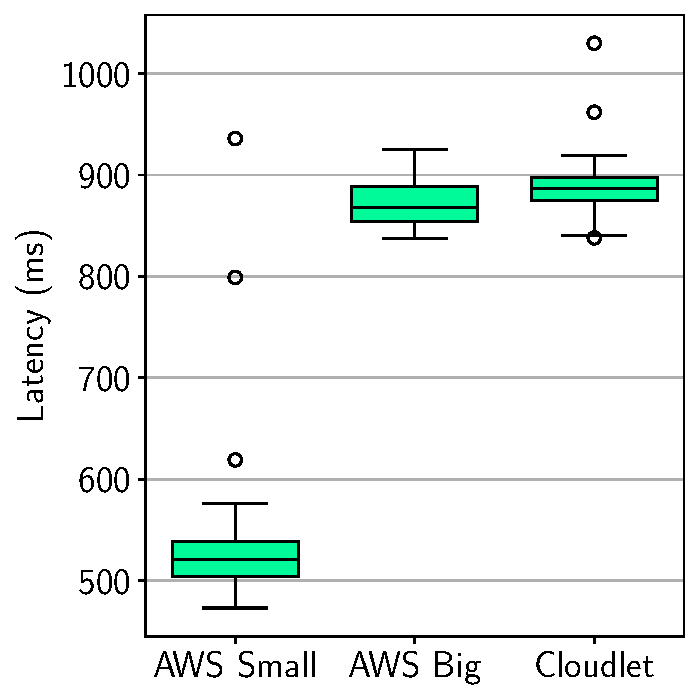
\includegraphics[height=2.5in]{figs/ffmpeg_box_plot.pdf}
        \caption{FFmpeg}
        \label{fig:ffmpeg_box_plot}
    \end{subfigure}
    \begin{subfigure}[t]{0.45\textwidth}
        \centering
        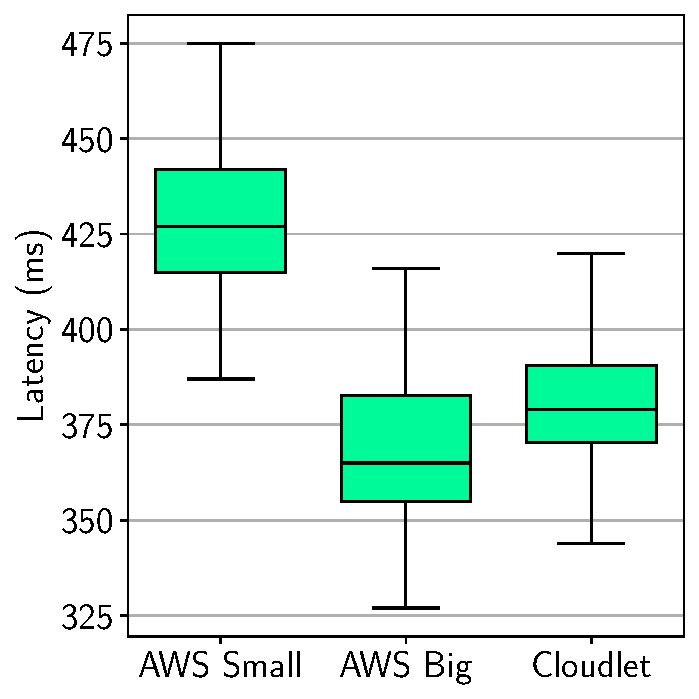
\includegraphics[height=2.5in]{figs/pdraw_box_plot.pdf}
        \caption{PDrAW}
        \label{fig:pdraw_box_plot}
    \end{subfigure}\vspace{1mm}\\
        \footnotesize{Each box extends from the first quartile ($Q_1$) to the third quartile ($Q_3$), with a line at the median. Whiskers extend from the box to the farthest data point lying within 1.5x the inter-quartile range ($IQR = Q_3-Q_1$) from the box. Circles represent outliers. 50 samples obtained for each configuration.}
    \caption{Latency Across Backend Locations Using Different Video Decoding Libraries}
    \label{fig:box_plots}
\end{figure}

This led to the hypothesis that FFmpeg's performance degrades with increased
parallelism, as it struggles to scale effectively with higher CPU counts.  To
test this hypothesis, measurements were obtained by varying the number of
threads used for FFmpeg from one to six (see \Cref{fig:threads_box_plot}).  The
OpenCV option \texttt{CAP\_\allowbreak PROP\_\allowbreak N\_\allowbreak
THREADS} was used to set the number of threads used for the FFmpeg backend.
The results show that the latency increases as we increase the number of threads,
suggesting that FFmpeg suffers from negative-scale out attributes. Adding more
threads to FFmpeg hurts latency.

\begin{figure}[htbp]
\centerline{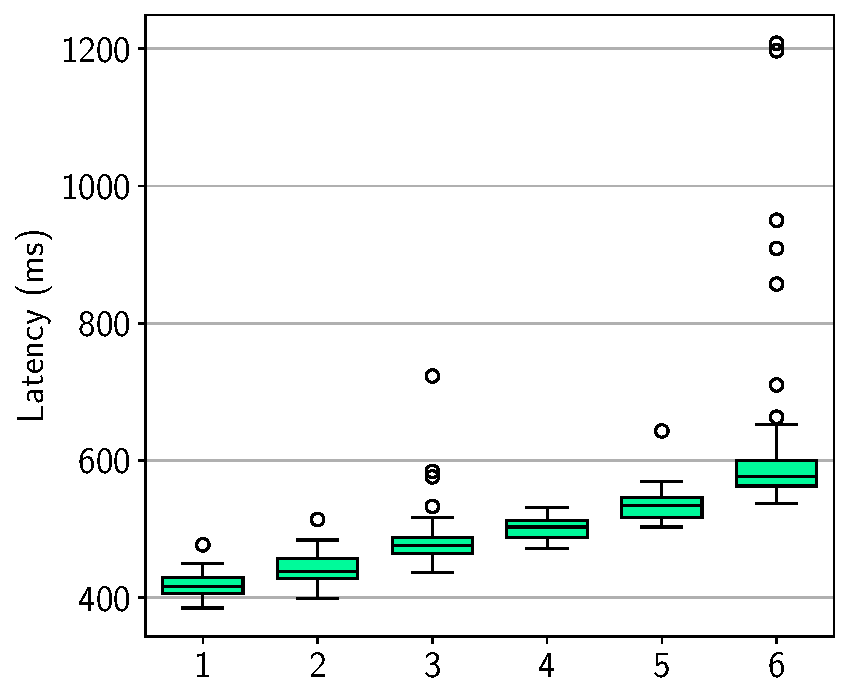
\includegraphics[width = .4\textwidth]{figs/threads_box_plot.pdf}}
\caption{Latency vs. Number of FFmpeg Threads}
\label{fig:threads_box_plot}
\end{figure}

Across all backend locations, we achieve the lowest latency by replacing FFmpeg
with PDrAW for video decoding.  For CMU Cloudlet, latency reduced
from 917 ms to 402 ms by switching to PDrAW, a speedup of almost 2.3$\times$.

\cref{fig:steeleagle_optimized_latency} shows the distribution of latency
obtained using our optimized configuration with PDrAW and the CMU cloudlet,
obtaining a mean of 380 ms and a 95th percentile latency of 402 ms.

\begin{figure}[htbp]
\centerline{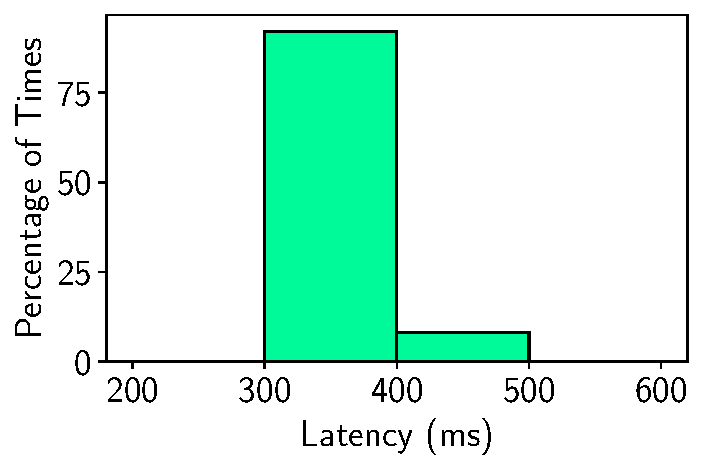
\includegraphics[width = .4\textwidth]{figs/pdraw_latency.pdf}}
\caption{Optimized SteelEagle Latency using PDrAW for Video Decoding}
\label{fig:steeleagle_optimized_latency}
\end{figure}

\section{Structured Benchmarking Using the OODA Loop Framework}
\label{sec:exp2}

\Cref{sec:exp1} covered an initial approach to benchmarking and optimizing the
SteelEagle pipeline, which only considered end-to-end drone-to-cloudlet
latency. It did not provide insight into the latency breakup of the pipeline
and where the new performance bottleneck resides. Several aspects of the
pipeline hinder obtaining this breakup.

The drone sensing and pre-processing, components (a) and (b) from
\cref{fig:ooda-mapping}, cannot be measured individually because the drone is a
COTS product that runs closed source software which does not allow the ability
to insert software instrumentation.  Similarly, drone post-processing and
actuation, components (f) and (g), must be measured together. Even measuring
components (a) and (b) in aggregate is challenging because of the way the Onion
Omega is used. Acting as a network gateway for the drone, the Onion Omega
routes network packets between the drone and the cloudlet. This is done by
establishing a VPN tunnel between the cloudlet and the Onion Omega using
WireGuard. The Onion Omega, in turn, connects to the drone's Wi-Fi hotspot,
allowing the cloudlet to reach the drone. There is no userspace application on
the Onion Omega where instrumentation can be inserted, the packet routing is
done by the kernel.

Another challenge involves measuring the video decoding time on the cloudlet,
part of component (d).  To measure decoding time, we need to measure the time
taken to receive the full decoded frame after the first network packet
corresponding to the frame arrived. A mapping from network packets to decoded
frames must be obtained to measure this. \Cref{fig:ooda-nomenclature} shows the
parts of the pipeline that can be measured in red: Oberve$_{ab}$, Observe$_c$,
Orient+Decide$_d$, Act$_e$, and Act$_{fg}$.

\begin{figure}[htbp]
    \centering
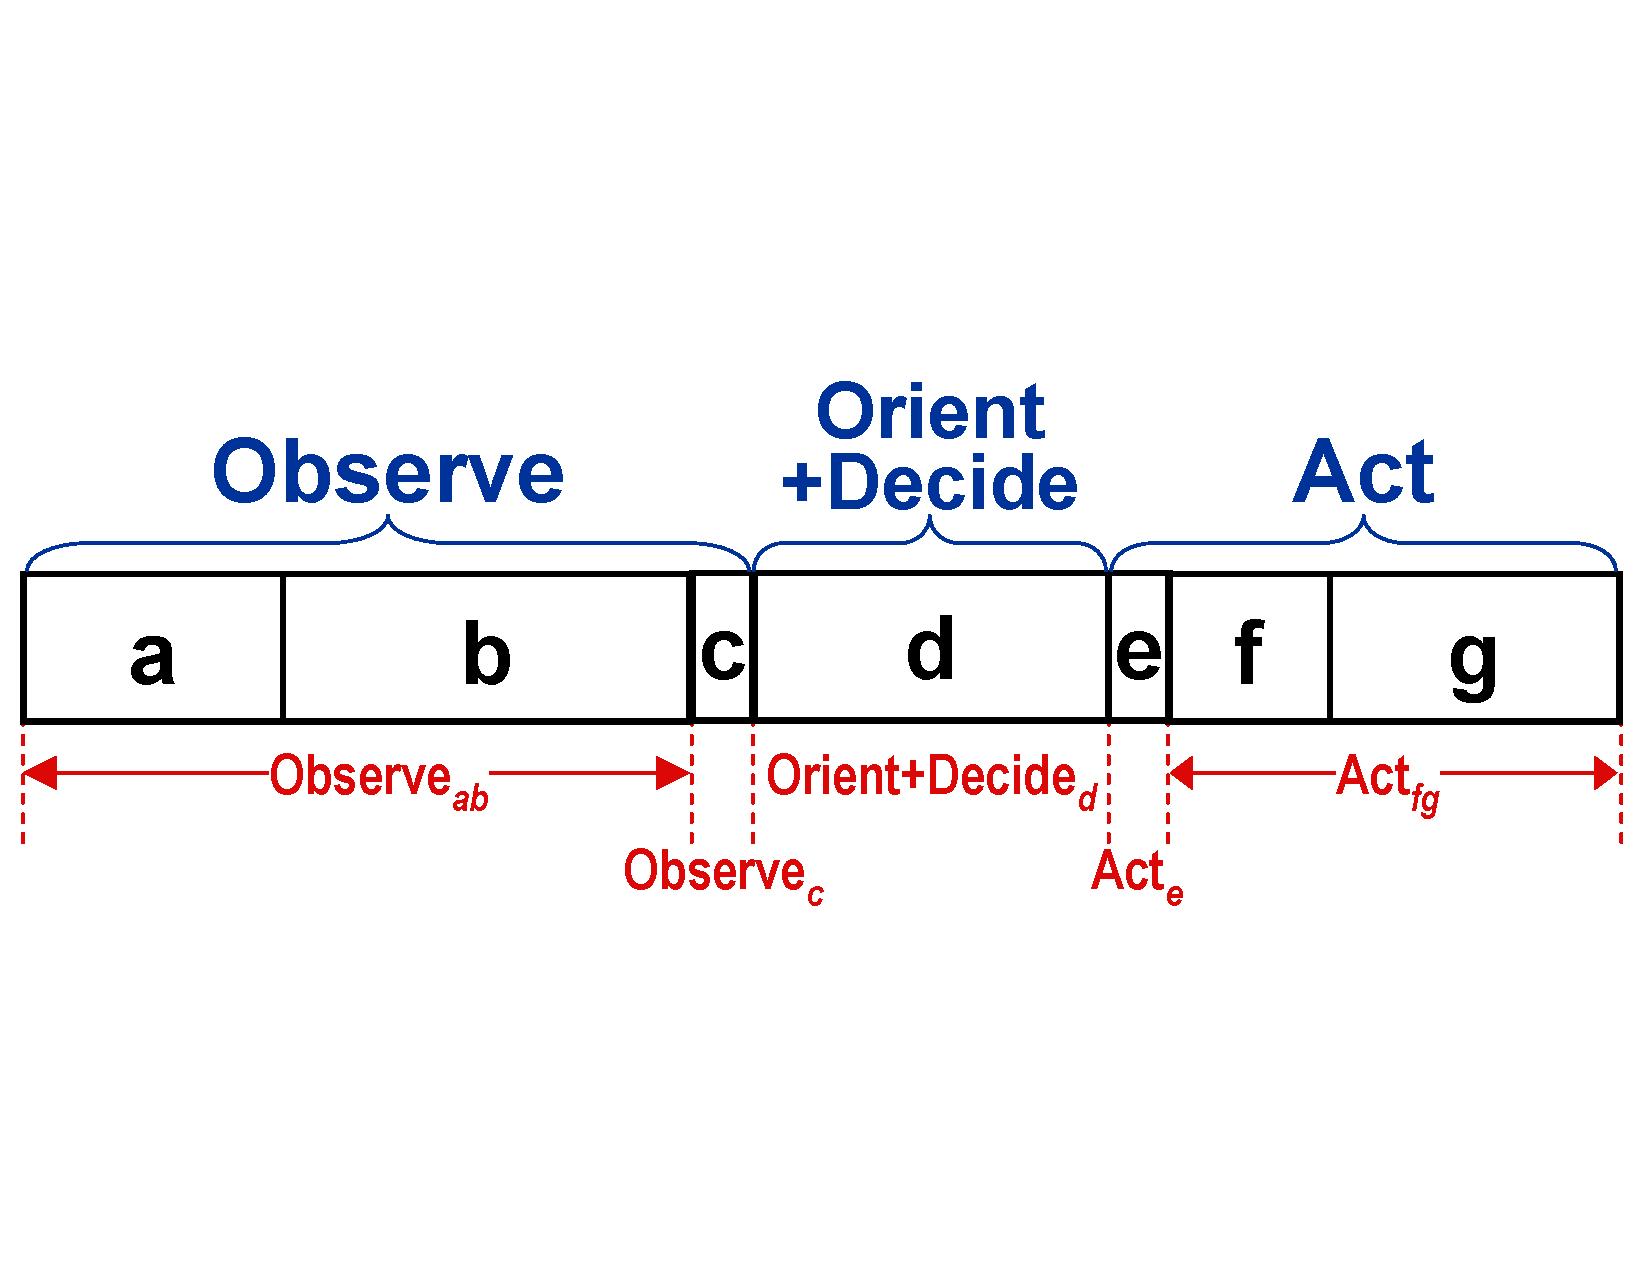
\includegraphics[width = .5\textwidth]{figs/fig-ooda-nomenclature.pdf}
	\begin{captext}
		\centering Only items in \textcolor{red}{red} above can be measured.
		\begin{tabular}{lll}
			\phantom{00} & a = on-drone sensing & e = transmission to drone\\
			\phantom{00} & b = on-drone pre-processing & f = on-drone post-processing\\
			\phantom{00} & c = transmission to cloudlet & g = drone actuation\\
			\phantom{00} & d = processing on cloudlet\\
		\end{tabular}
	\end{captext}
\caption{Measurable Components of the OODA Loop}
\label{fig:ooda-nomenclature}
\end{figure}

Our approach involves using the \texttt{tcpdump} program to capture network
packets on the Onion Omega and the cloudlet. As shown in
\cref{fig:exp2-method}, we record four timestamps, $t_1$ through $t_4$. $t_1$
corresponds to the Unix timestamp contained in the frame that the drone's
camera sees. $t_2$ is the timestamp of the first network packet transmitted by
the Onion Omega corresponding to this frame. $t_2-t_1$, then, corresponds to
Observe$_{ab}$.  $t_3$ is the time the first network packet corresponding to
this frame arrives at the cloudlet. $t_3-t_2$ is the network latency
Observe$_c$. Finally, $t_4$ is the timestamp recorded when this frame is
decoded on the cloudlet.  $t_4-t_3$ corresponds to the decoding time for this
frame, which is a part of Orient+Decide$_d$.

\begin{figure}[htbp]
    \centerline{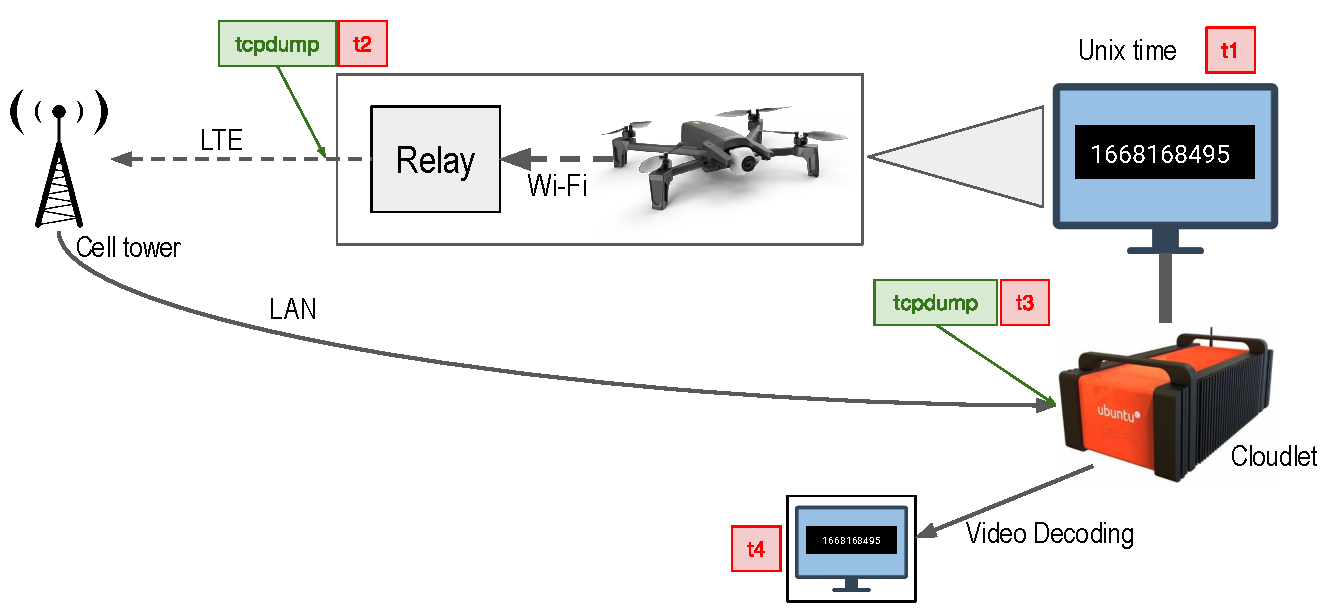
\includegraphics[width = .8\textwidth]{figs/fig-exp2-method-crop.pdf}}
    \caption{Obtaining Observe and Orient Latency using \texttt{tcpdump}}
\label{fig:exp2-method}
\end{figure}


\subsection{Obtaing a Correspondence between Network Packets and Frames}

To establish a correspondence between network packets and frames that is
required in this approach, we exploit the structure of the slice-encoded H.264
video stream transmitted by the drone\footnote{Credit to Qifei Dong, Ph.D.
student at Carnegie Mellon University, for devising this approach.}. Video
encoding formats typically includes two kinds of frames: intra-coded and
predicted.  Intra-coded frames, also known as I-frames, can be decoded
independently since they are self-contained. Predicted frames, or P-frames, are
decoded relative to a previous I-frame since they contain deltas calculated
using motion compensation techniques. In H.264 video encoding I-frames are sent
at a fixed periodicity, with a single I-frame sent in a group of pictures
(GOP), a unit defined as a fixed number of successive frames. In the presence
of network degradation, packet loss can cause a lost or incomplete I-frame to
affect the decoding of subsequent frames for the entire GOP.

To mitigate this, the Anafi drone performs video encoding at the slice level,
such that each 720p (1280x720) frame is divided into 45 slices, where each
slice is a 1280 pixels wide and 16 pixels high row of the frame.  I-frames and
P-frames become I-slice and P-slices in this slice-level encoding.  The video
encoding contains periodic I-slices to prevent error propogation, sending five
I-slices every three frames so that all slices are refreshed with an I-slice
every 27 frames (\cref{fig:slice-encoding}).

\begin{figure}[htbp]
    \centerline{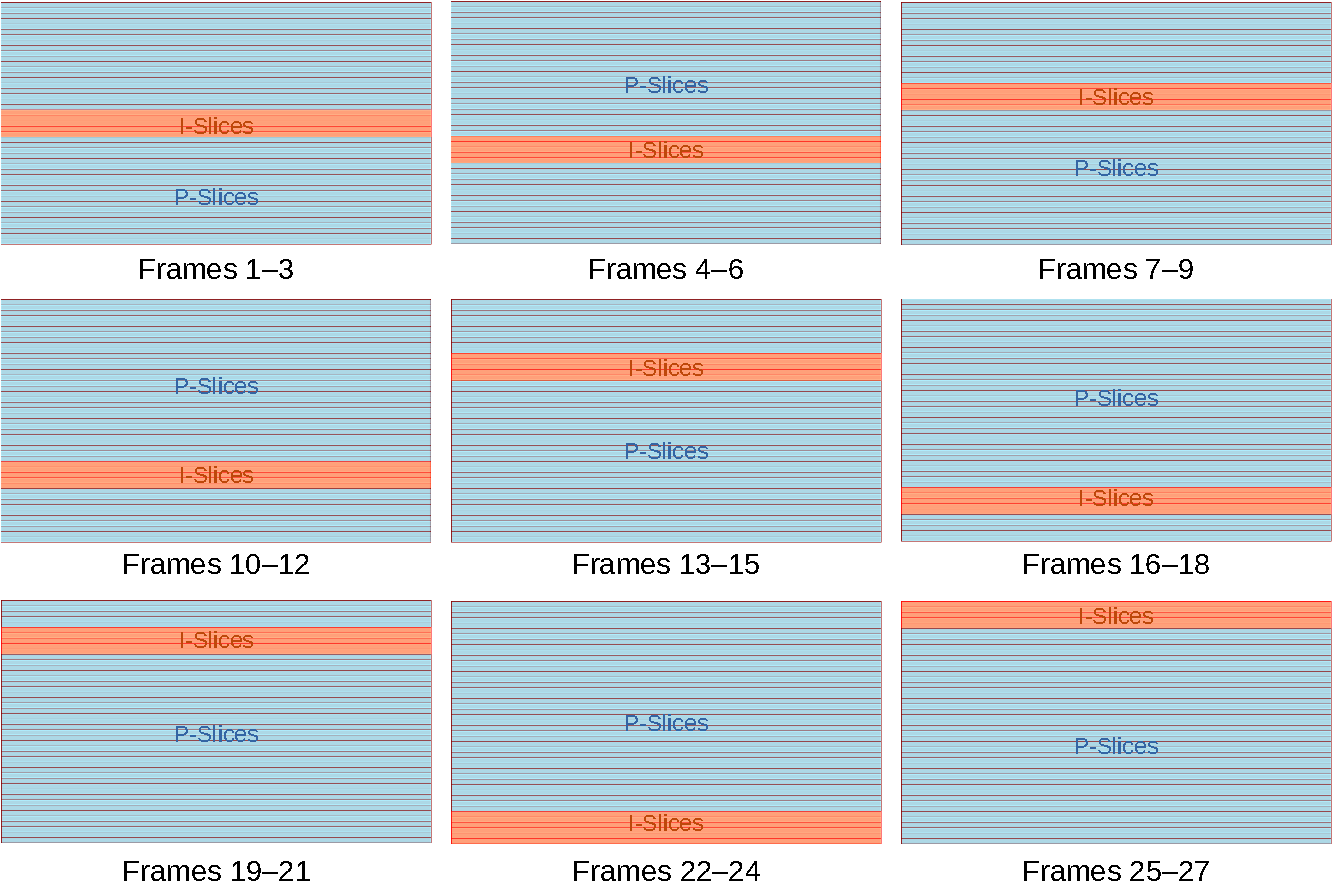
\includegraphics[width = .8\textwidth]{figs/fig-slice-encoding-crop.pdf}}
    \caption{The Anafi's Slice-Level Video Encoding Refresh Wave}
\label{fig:slice-encoding}
\end{figure}

Our approach temporarily filters network packets on the cloudlet originating
from the drone using the Linux kernel's \texttt{netfilter} framework. During
this time, the video decoder will miss the I-slices that it needs to decode
P-slices. After resuming packet flow, the video decoder will be temporarily
unable to correctly decode P-slices for which it missed an I-slice, leading to
degraded regions in the decoded frame. This degradation stops as new I-slices
are received during the refresh cycle, as the decoder only needs the latest
I-slices.

When packets are unfiltered, we can look for the first network packet that
contains an I-slice for a slice of our choosing. H.264 I-slices and P-slices
are encapsulated into Network Abstraction Layer Units (NALUs) when transmitted
over a network, which contains metadata that allows us to infer information
about the type of slice and the row that it corresponds to.

In practice, it is easier to filter network packets containing NALUs with
sequence parameter set (SPS) and picture parameter set (PPS) information, which
has general metadata related to the video stream, such as the video format.
This metadata is always sent along with the first frame in a GOP. Since the
first frame of the GOP contains the I-slice for rows 21 through 25 of the
frame, we need to identify the first frame that resolves degradations for these
rows.

In
\cref{fig:garbled-ts-1}, we see that the slice corresponding to the Unix
timestamp shown on the screen is degraded in the first few frames after we
unfilter UDP packets. Once we find the first network packet containing an
I-slice corresponding to this row, we can map it to the first frame outputted
by the decoder that resolves the degradation for that row
(\cref{fig:garbled-ts-2}).

\begin{figure}[htbp]
    \centering
    \begin{subfigure}[t]{0.45\textwidth}
        \centering
        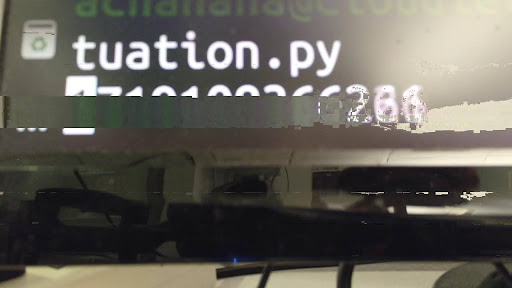
\includegraphics[width = \textwidth]{figs/garbled-ts-1.jpg}
        \caption{Degraded timestamp because of missed I-slice}
        \label{fig:garbled-ts-1}
    \end{subfigure}
    \hfill
    \begin{subfigure}[t]{0.45\textwidth}
        \centering
        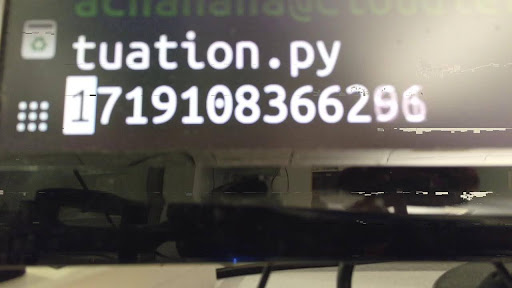
\includegraphics[width = \textwidth]{figs/garbel-ts-2.jpg}
        \caption{I-slice received for slice corresponding to timestamp}
        \label{fig:garbled-ts-2}
    \end{subfigure}
    \caption{Degraded Regions in Decoded Frame After Unfiltering UDP Packets}
\end{figure}

The kernel timestamps network packets, so we obtain $t_3$, the time the first
packet for frame \cref{fig:garbled-ts-2} arrived. Once a correspondance has
been establish between a network packet and a frame, we can look at the logical
timestamp that is associated with each frame during encoding and included in
each packet's metadata to obtain $t_3$ for subsequent frames---whenever the
logical timestamp increments, we know that the packet corresponds to the next
frame.

\subsection{Experimental Results}
\label{sec:measurements}

\subsubsection{\texorpdfstring{Observe$_{ab}$}{Observe\_ab}}
\label{sec:onion-observe-ab}

\begin{figure}[htbp]
    \centering
    \begin{subfigure}[t]{0.45\textwidth}
    \centering
    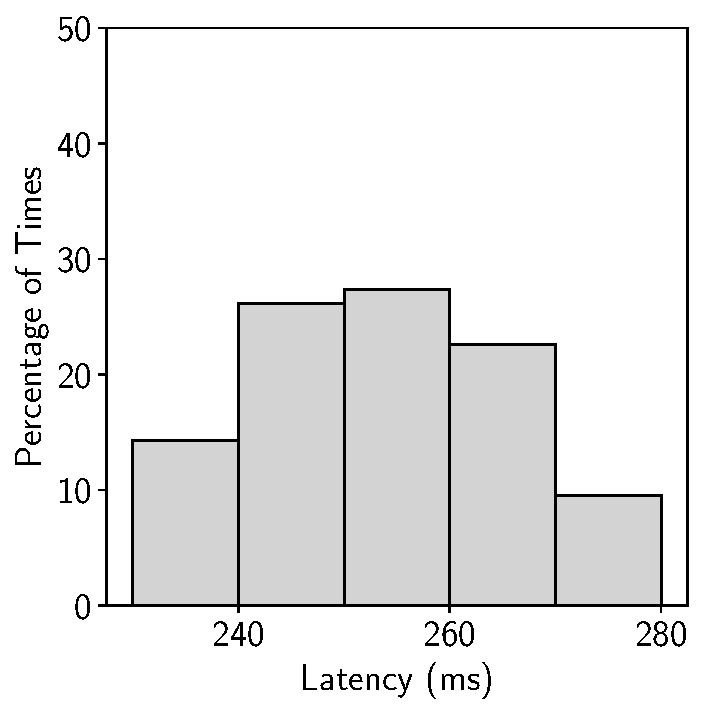
\includegraphics[width = .8\textwidth]{figs/observe-ab-latency.pdf}\\
    \small{Mean: 253.32$\pm$11.6~ms\; p99: 277.34~ms}\\
    \caption{Observe$_{ab}$ Latency}
    \label{fig:observe_ab_latency}
\end{subfigure}
\begin{subfigure}[t]{0.45\textwidth}
    \centerline{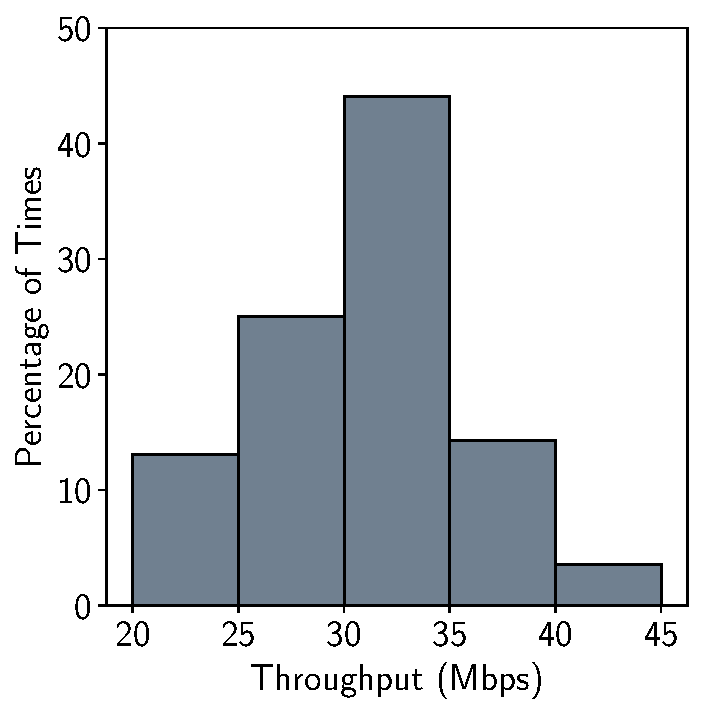
\includegraphics[width = .8\textwidth]{figs/observe-ab-throughput.pdf}}
    \centering
    \small{Mean: 30.83$\pm$4.95~fps\; p1: 22.1~fps}\\
    \caption{Observe$_{ab}$ Throughput}
    \label{fig:observe_ab_throughput}
\end{subfigure}
    \caption{Observe$_{ab}$ Measurements}
    \label{fig:observe_ab_measurements}
\end{figure}

\Cref{fig:observe_ab_measurements} shows that onboard drone sensing and
pre-processing, Observe$_{ab}$, has a mean latency of 253 ms, with a standard
deviation of 12 ms, and a p99 of 277 ms. Instantaneous throughput is also
measured in frames per second (fps), using the time taken for a new frame to be
transmitted by the drone. It has a mean of 31 fps, with a standard deviation of
5 fps and a p1 of 22 fps.

\subsubsection{\texorpdfstring{Observe$_c$}{Observe\_c}}

\begin{figure}[htbp]
    \centering
    \begin{subfigure}[t]{0.45\textwidth}
    \centering
    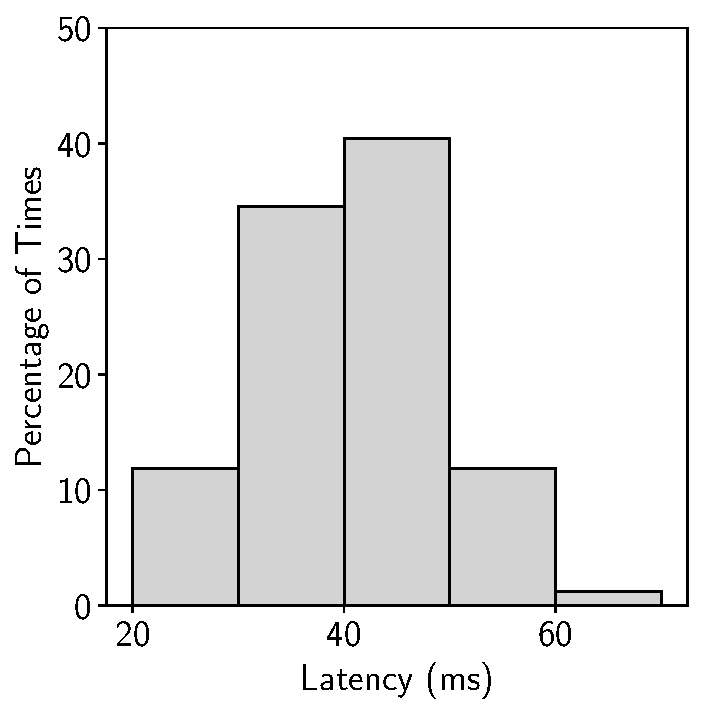
\includegraphics[width = .8\textwidth]{figs/observe-c-latency.pdf}\\
    \small{Mean: 39.37$\pm$8.07~ms\; p99: 59.51~ms}\\
    \caption{Observe$_{c}$ Latency}
    \label{fig:observe_c_latency}
\end{subfigure}
\begin{subfigure}[t]{0.45\textwidth}
    \centerline{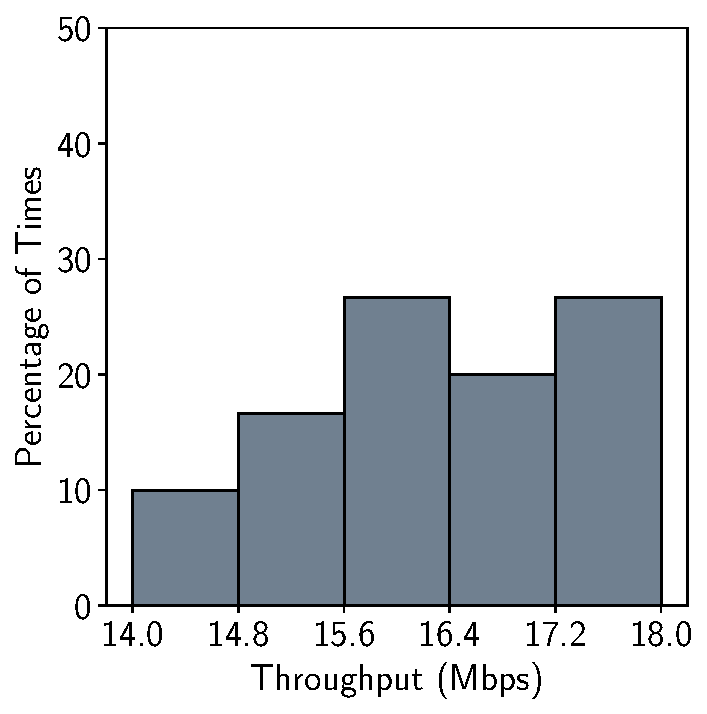
\includegraphics[width = .8\textwidth]{figs/observe-c-throughput.pdf}}
    \centering
    \small{Mean: 16.25$\pm$1.01~Mbps\; p1: 14.36~Mbps}\\
    \caption{Observe$_{c}$ Throughput}
    \label{fig:observe_c_throughput}
\end{subfigure}
    \caption{Observe$_{c}$ Measurements}
    \label{fig:observe_c_measurements}
\end{figure}

\Cref{fig:observe_c_measurements} shows the measurements obtained for
Observe$_c$, which involves transmission from the drone to the cloudlet. This
component includes a short Wi-Fi segment from the drone to the Onion Omega,
carried onboard the drone, and then a longer 4G LTE segment to the cloudlet.
Observe$_c$ has a mean latency of 39 ms, with a standard deviation of 8 ms, and
a p99 of 59 ms. The throughput measured on the link using \texttt{iperf} has a
mean of 16.25 Mbps, with a standard deviation of 1 Mbps and a p1 of 14.36 Mbps.

\subsubsection{\texorpdfstring{Orient+Decide$_d$}{Orient+Decide\_d}}
\label{sec:onion-orient-decide-d}

\begin{figure}[htbp]
    \centering
    \begin{subfigure}[t]{0.45\textwidth}
    \centering
    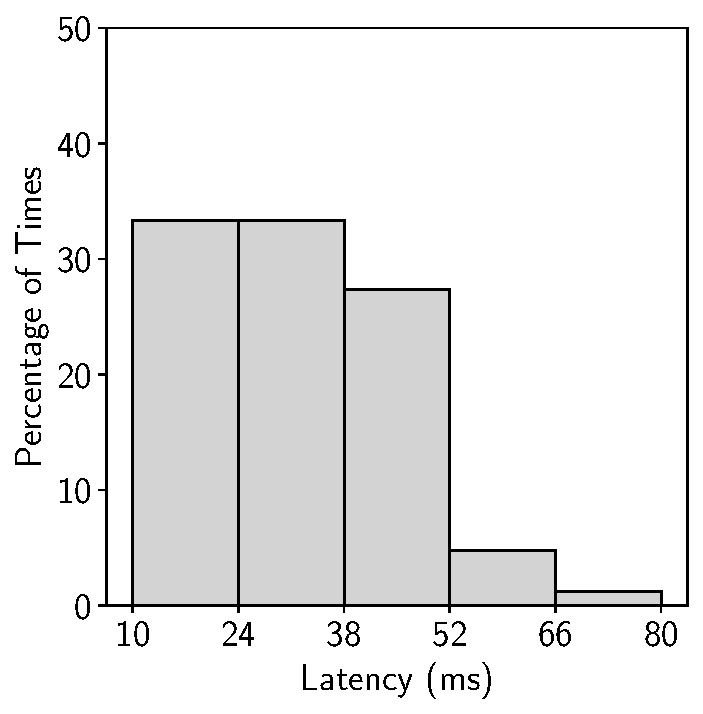
\includegraphics[width = .8\textwidth]{figs/stage-1-latency-pdraw.pdf}\\
    \small{Mean: 32.26$\pm$12.75~ms\; p99: 59.08~ms}\\
    \caption{Orient+Decide$_{d}$ Latency}
    \label{fig:stage1_latency}
\end{subfigure}
\begin{subfigure}[t]{0.45\textwidth}
    \centerline{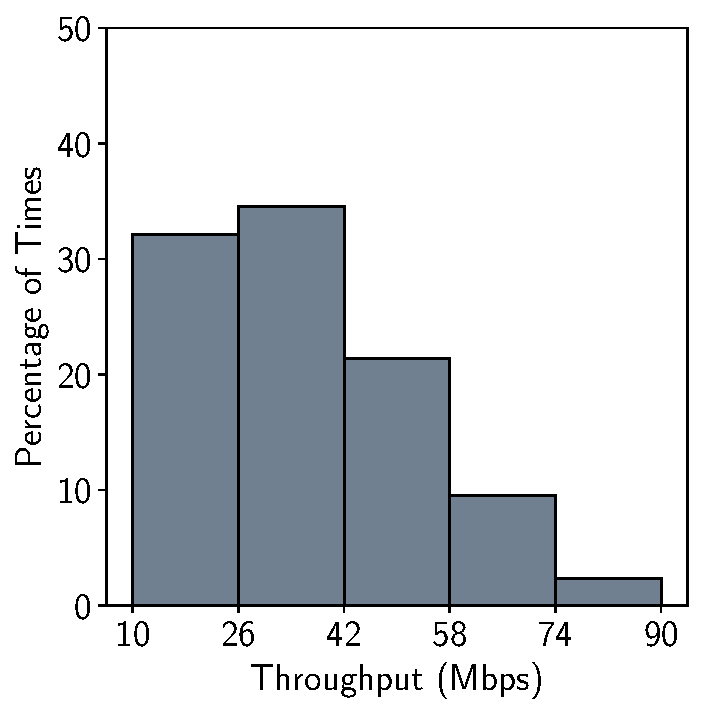
\includegraphics[width = .8\textwidth]{figs/stage-1-throughput-pdraw.pdf}}
    \centering
    \small{Mean: 36.57$\pm$15.88~fps\; p1: 17.24~fps}\\
    \caption{Orient+Decide$_{d}$ Throughput}
    \label{fig:stage1_throughput}
\end{subfigure}
    \caption{Orient+Decide$_{d}$ Measurements}
    \label{fig:stage1_measurements}
\end{figure}

\Cref{fig:stage1_measurements} presents the latency and throughput measurements
for Orient+Decide$_d$. This component includes three stages:

\begin{itemize}
    \item \textbf{Stage 1.} Decoding of the drone's RTSP H.264 video stream to produce
    individual frames
\item \textbf{Stage 2.} Inferencing on each frame. This could involve using a deep
    neural network (DNN) to perform tasks such as depth estimation or object
    detection.
\item \textbf{Stage 3.} Determining drone actuation needed based on findings from Stage
    2 and generating the corresponding command.
\end{itemize}

Stage 2 and Stage 3's performance can vary depending on the application.
Different DNNs can have different inference times, and the decision logic can
vary in complexity.  Stage 1, however, remains the same and so we focus on
measuring Stage 1 for Observe+Decide$_d$. We see a mean latency of 32 ms for
Stage 1, with a standard deviation of 13 ms, and a p99 of 59 ms. The decoding
software's throughput was measured as the inverse of its latency, giving an
indication of the frame rate that the decoding software can sustain on our
cloudlet hardware. The throughput has a mean of 37 fps with a standard
deviation of 17 fps and a p1 of 17 fps.

\subsubsection{\texorpdfstring{Act$_e$}{Act\_e}}

\begin{figure}[htbp]
    \centering
    \begin{subfigure}[t]{0.45\textwidth}
    \centering
    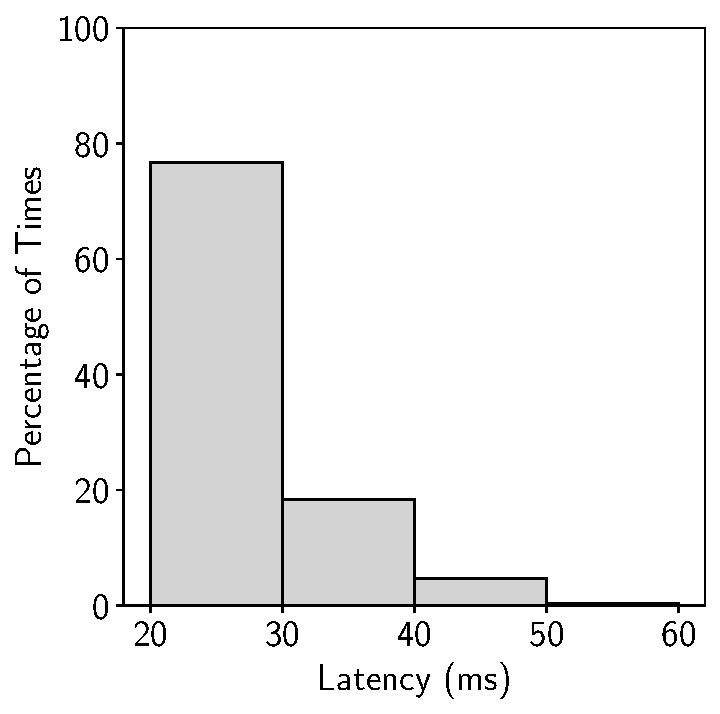
\includegraphics[width = .8\textwidth]{figs/act-e-latency.pdf}\\
    \small{Mean: 30$\pm$4.22~ms\; p99: 49~ms}\\
    \caption{Act$_{e}$ Latency}
    \label{fig:act-e-latency}
\end{subfigure}
\begin{subfigure}[t]{0.45\textwidth}
    \centerline{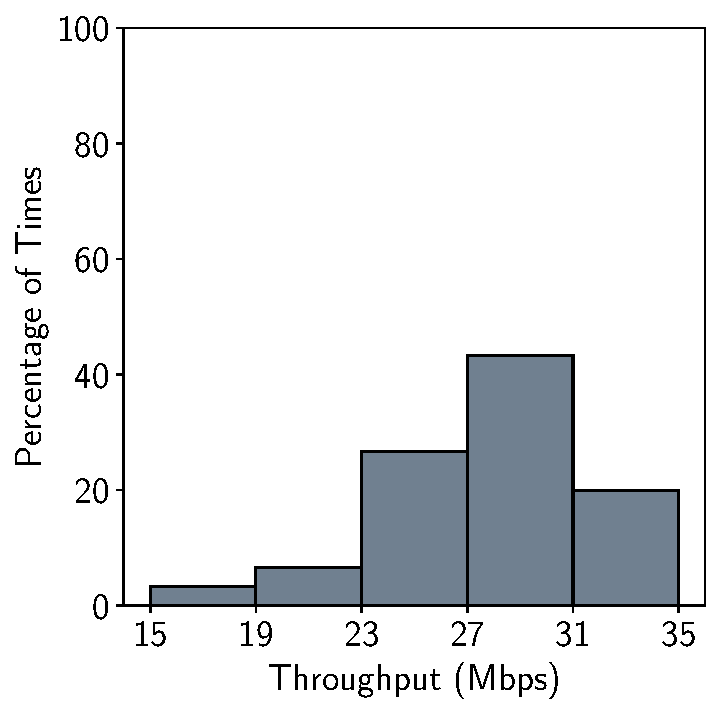
\includegraphics[width = .8\textwidth]{figs/act-e-throughput.pdf}}
    \centering
    \small{Mean: 28$\pm$3.66~Mbps\; p1: 19~Mbps}\\
    \caption{Act$_{e}$ Throughput}
    \label{fig:act-e-throughput}
\end{subfigure}
    \caption{Act$_{e}$ Measurements}
    \label{fig:act_e_measurements}
\end{figure}

\Cref{fig:act_e_measurements} shows the measurements for Act$_e$, which
involves the transmission of drone actuation commands back to the drone via the
Onion Omega. This is the return path of Observe$_c$, and involves a 4G LTE and
Wi-Fi segment as before. Since drone commands have a small data size, latency
is a more crucial aspect of this component. Nevertheless, bandwidth for Act$_e$
is much higher than Observe$_c$ because for the Onion Omega it corresponds to
4G LTE downlink, which offers a higher bandwidth than uplink because mobile
networks are designed to optimize downlink performance.

The latency has a mean of 30 ms, with a standard deviation of 4.22 ms and a
p99 of 49 ms. The throughput has a mean of 28 Mbps, with a standard deviation
of 3.66 Mbps and a p1 of 19 Mbps.

\subsubsection{\texorpdfstring{Act$_{fg}$}{Act\_fg}}
\label{sec:onion-act-fg}

\begin{wrapfigure}[12]{r}{0.3\linewidth}
\centering
%\includegraphics[width=0.45\linewidth]{FIGS/act_latency.png}
    \begin{tabular}{@{}cc@{}}
\toprule
Run & Latency (ms)\\
\midrule
 1&188\\
 2&170\\
 3&162\\
 4&189\\
 5&155\\
\midrule
Mean& 173~{\small$\pm$15}\\
\bottomrule
\end{tabular}
\caption{\small Act$_{fg}$  Latency}
\label{fig:act-fg-latency}
\end{wrapfigure}
Act$_{fg}$ involves processing of an actuation command by the drone and the
initiation of actuation. We measure the latency as the time difference between
the receipt of an actuation command by the drone and the start of actuation.
To measure this, we position a stationary drone in front of a display connected
to the cloudlet showing the current timestamp at millisecond granularity.  An
actuation command is sent to the drone to move its gimbal while the display and
gimbal are video-recorded using a slow-motion camera. We output the timestamp
at which the actuation command is sent and identify the first video frame
showing gimbal movement. Act$_{fg}$ latency is calculated as the difference
between the timestamp shown on the display in this frame and the timestamp at
which the drone acutation command was sent. \Cref{fig:act-fg-latency} shows
that Act$_{fg}$ has a mean latency of 173 ms, with a standard deviation of 15
ms.  We use a slow-motion camera which operates at 240 fps, resulting in a
frame interval of approximately 4 ms. The measurements have an error margin of
about five frames, resulting in an experimental error of approximately 20 ms.

Act$_{fg}$ involves electromechanical actuation, which does not have a concept
of streaming. As a result, throughput can be interpreted as the reciprocal of
latency.

\subsection{Overview of OODA Loop}

\begin{figure}[htbp]
    \centerline{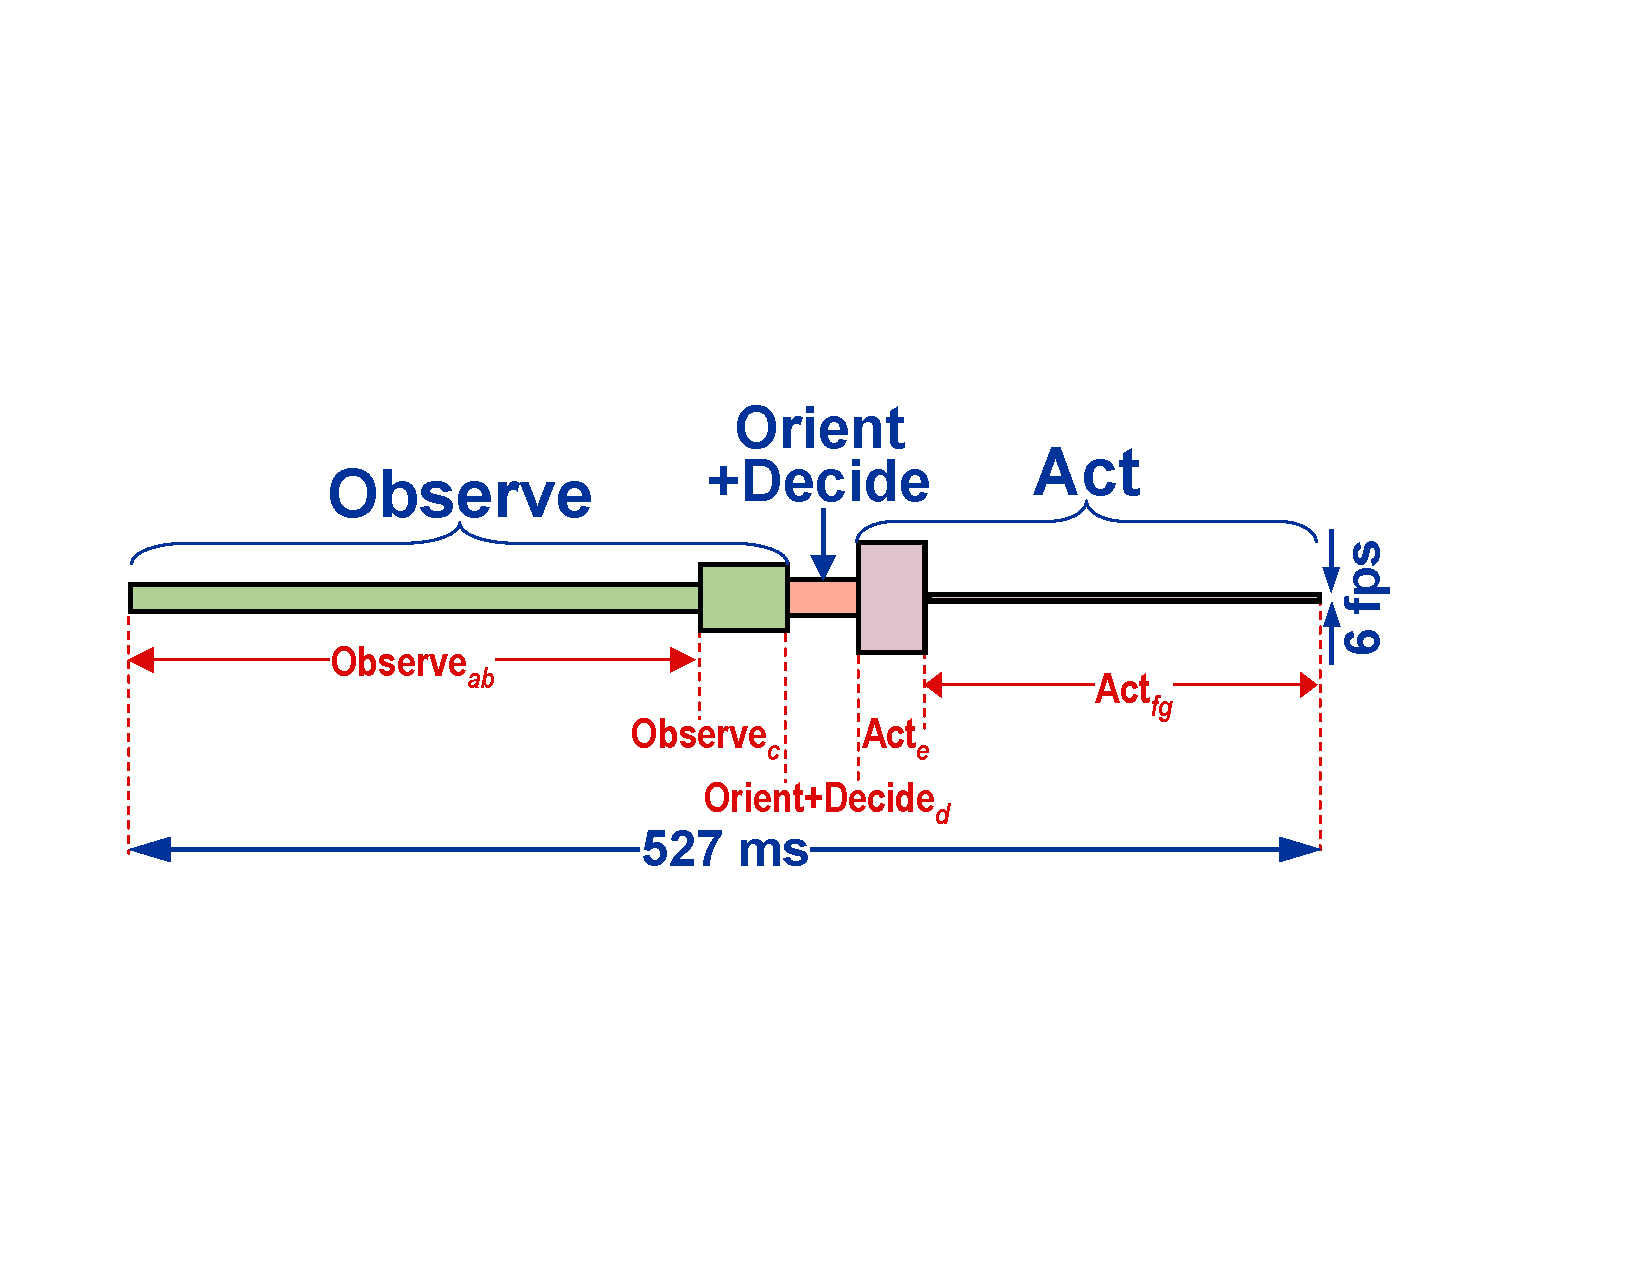
\includegraphics[width = .6\textwidth]{figs/fig-ooda-scaling.pdf}}
    \caption{SteelEagle OODA Loop Throughput and Latency Overview}
\label{fig:ooda-scaling}
\end{figure}

\Cref{fig:ooda-scaling} presents a summary of the measurements from
\cref{sec:measurements}. This depiction shows that in the best case, assuming
no time is spent on Stage 2 and Stage 3 in the Orient+Decide$_d$ component, the
drone takes 527 ms to react to a change in its environment. In practice, Stage
2 and Stage 3 can involve complex computationally-intensive inferencing and
decision-making, such as the use of DNNs for depth estimation or object
tracking, and route planning algorithms. The height and width of the
Orient+Decide$_d$ component in \cref{fig:ooda-scaling} would need to be scaled
appropriately to account for this.

\chapter{Section 1}

We have discussed many things.
But, it is unclear we have really discussed the nature of them.

\section{More things}

\subsection{Moore things}

We can even put a picture in here, which is harder than it looks.

\begin{figure}[htbp]
\centerline{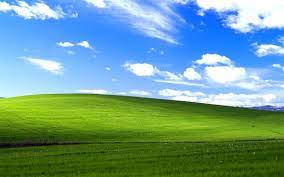
\includegraphics[width = .85\textwidth]{Unknown.jpeg}}
\caption{Something}
\label{fig}
\end{figure}
\chapter{Section 2}

We have derived the basics of things.
Now let us look at the things themselves.

\section{The things are alive}

This is a table.

\begin{table}[h!]
\centering
\begin{tabular}{ |p{1cm}||p{2cm}|p{2cm}|p{5cm}|p{3cm}| }
 \hline
 \multicolumn{5}{|c|}{Table of things that are alive} \\
 \hline
 T & H & i & N & G \\
 \hline
 Alps   & 0  & 5 &  e & hovercraft\\
 16   & dog  & 5 &  e & 80\\
 32   & 0  & pangolin &  l & 210\\
 M   & 0  & 5 &  s & 810\\
 \hline
\end{tabular}
\caption{Table to test captions and labels}
\label{table:1}
\end{table}
\chapter{Conclusion and Future Work}
\section{Conclusion}
Tell me
\section{Future Work}



%\appendix
%\include{appendix}

\backmatter
%\renewcommand{\baselinestretch}{1.0}\normalsize

% By default \bibsection is \chapter*, but we really want this to show
% up in the table of contents and pdf bookmarks.
\renewcommand{\bibsection}{\chapter{\bibname}}
%\newcommand{\bibpreamble}{This text goes between the ``Bibliography''
%  header and the actual list of references}
\bibliographystyle{unsrt}
\bibliography{register} %your bib file

% \begin{thebibliography}{00}
%
% \bibitem{thing} thing
%
% \end{thebibliography}

\end{document}
